%% 使用 njuthesis 文档类生成南京大学学位论文的示例文档
%%
%% 作者:胡海星,starfish (at) gmail (dot) com
%% 项目主页: http://haixing-hu.github.io/nju-thesis/
%%
%% 本样例文档中用到了吕琦同学的博士论文的提高和部分内容,在此对他表示感谢。
%%
\documentclass[macfonts,master]{njuthesis}
%% njuthesis 文档类的可选参数有:
%%   nobackinfo 取消封二页导师签名信息。注意,按照南大的规定,是需要签名页的。
%%   phd/master/bachelor 选择博士/硕士/学士论文

% 使用 blindtext 宏包自动生成章节文字
% 这仅仅是用于生成样例文档,正式论文中一般用不到该宏包
\usepackage[math]{blindtext}
\usepackage{setspace}

%%%%%%%%%%%%%%%%%%%%%%%%%%%%%%%%%%%%%%%%%%%%%%%%%%%%%%%%%%%%%%%%%%%%%%%%%%%%%%%
% 设置《国家图书馆封面》的内容,仅博士论文才需要填写

% 设置论文按照《中国图书资料分类法》的分类编号
\classification{0175.2}
% 论文的密级。需按照GB/T 7156-2003标准进行设置。预定义的值包括:
% - \openlevel,表示公开级:此级别的文献可在国内外发行和交换。
% - \controllevel,表示限制级:此级别的文献内容不涉及国家秘密,但在一定时间内
%   限制其交流和使用范围。
% - \confidentiallevel,表示秘密级:此级别的文献内容涉及一般国家秘密。
% - \clasifiedlevel,表示机密级:此级别的文献内容涉及重要的国家秘密 。
% - \mostconfidentiallevel,表示绝密级:此级别的文献内容涉及最重要的国家秘密。
% 此属性可选,默认为\openlevel,即公开级。
\securitylevel{\controllevel}
% 设置论文按照《国际十进分类法UDC》的分类编号
% 该编号可在下述网址查询:http://www.udcc.org/udcsummary/php/index.php?lang=chi
\udc{004.72}
% 国家图书馆封面上的论文标题第一行,不可换行。此属性可选,默认值为通过\title设置的标题。
\nlctitlea{数据中心}
% 国家图书馆封面上的论文标题第二行,不可换行。此属性可选,默认值为空白。
\nlctitleb{网络模型研究}
% 国家图书馆封面上的论文标题第三行,不可换行。此属性可选,默认值为空白。
\nlctitlec{}
% 导师的单位名称及地址
\supervisorinfo{南京大学计算机科学与技术系~~南京市汉口路22号~~210093}
% 答辩委员会主席
\chairman{张三丰~~教授}
% 第一位评阅人
\reviewera{阳顶天~~教授}
% 第二位评阅人
\reviewerb{张无忌~~副教授}
% 第三位评阅人
\reviewerc{黄裳~~教授}
% 第四位评阅人
\reviewerd{郭靖~~研究员}

%%%%%%%%%%%%%%%%%%%%%%%%%%%%%%%%%%%%%%%%%%%%%%%%%%%%%%%%%%%%%%%%%%%%%%%%%%%%%%%
% 设置论文的中文封面

% 论文标题,不可换行
\title{支持事务一致性的微服务动态更新系统实现}
% 如果论文标题过长,可以分两行,第一行用\titlea{}定义,第二行用\titleb{}定义,将上面的\title{}注释掉
% \titlea{半轻衰变$D^+\to \omega(\phi)e^+\nu_e$的研究}
% \titleb{和弱衰变$J/\psi \to D_s^{(*)-}e^+\nu_e$的寻找}

% 论文作者姓名
\author{王东宇}
% 论文作者联系电话
\telphone{18362926576}
% 论文作者电子邮件地址
\email{wdongyu@outlook.com}
% 论文作者学生证号
\studentnum{MG1833071}
% 论文作者入学年份(年级)
\grade{2018}
% 导师姓名职称
\supervisor{曹春~~教授}
% 导师的联系电话
\supervisortelphone{18951679203}
% 论文作者的学科与专业方向
\major{计算机科学与技术}
% 论文作者的研究方向
\researchfield{软件方法学}
% 论文作者所在院系的中文名称
\department{计算机科学与技术系}
% 论文作者所在学校或机构的名称。此属性可选,默认值为``南京大学''。
\institute{南京大学}
% 论文的提交日期,需设置年、月、日。
\submitdate{2021年4月115日}
% 论文的答辩日期,需设置年、月、日。
\defenddate{2021年6月1日}
% 论文的定稿日期,需设置年、月、日。此属性可选,默认值为最后一次编译时的日期,精确到日。
%% \date{2013年5月1日}

%%%%%%%%%%%%%%%%%%%%%%%%%%%%%%%%%%%%%%%%%%%%%%%%%%%%%%%%%%%%%%%%%%%%%%%%%%%%%%%
% 设置论文的英文封面

% 论文的英文标题,不可换行
\englishtitle{Implementation of a Microservice System Supporting Dynamic Update With Transaction Consistency}
% 论文作者姓名的拼音
\englishauthor{Dongyu Wang}
% 导师姓名职称的英文
\englishsupervisor{Professor Chun Cao}
% 论文作者学科与专业的英文名
\englishmajor{Computer Science and Technology}
% 论文作者所在院系的英文名称
\englishdepartment{Department of Computer Science and Technology}
% 论文作者所在学校或机构的英文名称。此属性可选,默认值为``Nanjing University''。
\englishinstitute{Nanjing University}
% 论文完成日期的英文形式,它将出现在英文封面下方。需设置年、月、日。日期格式使用美国的日期
% 格式,即``Month day, year'',其中``Month''为月份的英文名全称,首字母大写;``day''为
% 该月中日期的阿拉伯数字表示;``year''为年份的四位阿拉伯数字表示。此属性可选,默认值为最后
% 一次编译时的日期。
\englishdate{April 15, 2021}

%%%%%%%%%%%%%%%%%%%%%%%%%%%%%%%%%%%%%%%%%%%%%%%%%%%%%%%%%%%%%%%%%%%%%%%%%%%%%%%
% 设置论文的中文摘要

% 设置中文摘要页面的论文标题及副标题的第一行。
% 此属性可选,其默认值为使用|\title|命令所设置的论文标题
\abstracttitlea{支持事务一致性的微服务动态更新系统实现}
% 设置中文摘要页面的论文标题及副标题的第二行。
% 此属性可选,其默认值为空白
% \abstracttitleb{}

%%%%%%%%%%%%%%%%%%%%%%%%%%%%%%%%%%%%%%%%%%%%%%%%%%%%%%%%%%%%%%%%%%%%%%%%%%%%%%%
% 设置论文的英文摘要

% 设置英文摘要页面的论文标题及副标题的第一行。
% 此属性可选,其默认值为使用|\englishtitle|命令所设置的论文标题
\englishabstracttitlea{Implementation of a Microservice System Supporting}
% 设置英文摘要页面的论文标题及副标题的第二行。
% 此属性可选,其默认值为空白
\englishabstracttitleb{Dynamic Update With Transaction Consistency}

%%%%%%%%%%%%%%%%%%%%%%%%%%%%%%%%%%%%%%%%%%%%%%%%%%%%%%%%%%%%%%%%%%%%%%%%%%%%%%%
\begin{document}

%%%%%%%%%%%%%%%%%%%%%%%%%%%%%%%%%%%%%%%%%%%%%%%%%%%%%%%%%%%%%%%%%%%%%%%%%%%%%%%

% 制作国家图书馆封面(博士学位论文才需要)
% \makenlctitle
% 制作中文封面
\maketitle
% 制作英文封面
\makeenglishtitle


%%%%%%%%%%%%%%%%%%%%%%%%%%%%%%%%%%%%%%%%%%%%%%%%%%%%%%%%%%%%%%%%%%%%%%%%%%%%%%%
% 开始前言部分
\frontmatter

%%%%%%%%%%%%%%%%%%%%%%%%%%%%%%%%%%%%%%%%%%%%%%%%%%%%%%%%%%%%%%%%%%%%%%%%%%%%%%%
% 论文的中文摘要
\begin{abstract}
基于微服务架构(Microservices Architecture)的开发可以有效地缩短开发周期,满足了软件快速持续集成和持续交付的需求,在工业界得到广泛的应用。已部署的软件通常需要不断地进行更新迭代,以达到漏洞修复、增强功能以及适应外部需求等多方面的目的。然而传统的更新方式通常需要停止系统、部署新版本后再重新启动系统。很多关键领域的系统并不能接受停机更新所导致的系统中断,因此软件动态更新技术显得尤为关键。

当前相关的微服务框架与架构对服务的动态更新支撑不足,没有考虑动态更新过程中系统的一致性。基于此,本文给出了一种支持事务一致性的微服务动态更新方法,并在具体的微服务架构上进行模型的扩展,完成了系统的设计与实现。此外,将本文的方法与实际的应用案例进行整合,完成了此方法和相关更新算法的实验评估对比,验证了其在更新过程中的安全性、及时性和低干扰性,以及对多服务同时进行更新的支持。

具体而言,本文的工作主要包括:\\

\begin{spacing}{1.0}
\end{spacing}

$\bullet$分析当前主流微服务框架技术在动态更新支撑方面的不足。针对此不足

$\indent\enspace$,提出一种支持事务一致性的微服务动态更新的实现方法,在事务模型

$\indent\enspace$、动态依赖管理和服务生命周期三个方面进行了相应的扩展,为具体的

$\indent\enspace$动态更新过程提供运行时支持。

\begin{spacing}{2.0}
\end{spacing}

$\bullet$基于上述的实现方法,在开源实现框架Istio之上完成了模型的扩展,添

$\indent\enspace$加系统对动态更新的支持。该系统不仅保证动态更新过程的安全性、及

$\indent\enspace$时性和低干扰性,而且实现的扩展模块对用户保持透明,与具体的服务

$\indent\enspace$业务逻辑解耦开。

\begin{spacing}{2.0}
\end{spacing}

$\bullet$利用实际的应用案例,整合上述实现方法并进行实验评估。通过使用不

$\indent\enspace$同的更新算法,主要对动态更新过程中各个算法的安全性(Safety)、及

$\indent\enspace$时性(Timeliness)、干扰性(Disruption)进行了性能比较,具体实验中同

$\indent$$\enspace$时向多个服务发起动态更新请求,验证了本文实现方法对于多服务同时

$\indent$$\enspace$更新的可行性和有效性。\\

\begin{spacing}{1.0}
\end{spacing}

% 中文关键词。关键词之间用中文全角分号隔开,末尾无标点符号。
\keywords{微服务架构;事务一致性;动态更新}
\end{abstract}

%%%%%%%%%%%%%%%%%%%%%%%%%%%%%%%%%%%%%%%%%%%%%%%%%%%%%%%%%%%%%%%%%%%%%%%%%%%%%%%
% 论文的英文摘要
\begin{englishabstract}
Development based on the microservices architecture can effectively shorten the development cycle, meet the needs of rapid continuous integration and continuous delivery of software, and is widely used in the industry. The deployed software often need to be updated continuously to achieve various purposes such as bug fixes, enhancements, and adaptation to external requirements. However, the traditional way to update a software system is to stop the system, replace it with the new version, then restart it. This is not acceptable for some mission critical system for the interruption caused by downtime updates, so in such situations we need dynamic software update(DSU).

Existing microservice framework and architecture provide limited supports for DSU, and do not take in account the system consistency during the dynamic update process. Based on this, this thesis presents a method for microservices that supports dynamic update with transaction consistency, extends the models on specific microservice architecture, and completes the design and implementation of the system. We have also integrated the method with the actual application case, completed the experimental evaluation and comparison with the related update algorithm, and the safety, update timeliness and low disruption during the update process , as well as support for simultaneous updates of multiple services are verified. 

The main work can be summarized as follows: 

\begin{itemize}
  \item This thesis analyze the deficiencies of the existing microservice framework in dynamic update support. To solve this problem, we present a method for microservices that supports dynamic update with transaction consistency. It extends the transaction model, dynamic dependency management and service lifecycle to provide runtime support for specific dynamic update process.
  \item Based on the implementation method, the model is extended on the open source implementation framework Istio and support for dynamic update is added. The system not only ensure the safety, update timeliness and low disruption of the dynamic update process, but also the extension modules remain transparent to users and decoupled from the specific service business logic.
  \item We have chosen a practical application case to integrate the implementation method and conduct experimental evaluations. Through the use of various update algorithms, the focus is put on the safety, update timeliness and disruption. In the specific experiment, dynamic update requests are initiated to multiple services at the same time, which verified the feasibility and effectiveness of the method implemented in this paper for multi services simultaneous update.
\end{itemize}
% 英文关键词。关键词之间用英文半角逗号隔开,末尾无符号。
\englishkeywords{Microservices Architecture, Transaction Consistency, Dynamic Update}
\end{englishabstract}

%%%%%%%%%%%%%%%%%%%%%%%%%%%%%%%%%%%%%%%%%%%%%%%%%%%%%%%%%%%%%%%%%%%%%%%%%%%%%%%
% 论文的前言,应放在目录之前,中英文摘要之后

%%%%%%%%%%%%%%%%%%%%%%%%%%%%%%%%%%%%%%%%%%%%%%%%%%%%%%%%%%%%%%%%%%%%%%%%%%%%%%%
% 生成论文目次
\tableofcontents

%%%%%%%%%%%%%%%%%%%%%%%%%%%%%%%%%%%%%%%%%%%%%%%%%%%%%%%%%%%%%%%%%%%%%%%%%%%%%%%
% 生成插图清单。如无需插图清单则可注释掉下述语句。
\listoffigures

%%%%%%%%%%%%%%%%%%%%%%%%%%%%%%%%%%%%%%%%%%%%%%%%%%%%%%%%%%%%%%%%%%%%%%%%%%%%%%%
% 生成附表清单。如无需附表清单则可注释掉下述语句。
\listoftables

%%%%%%%%%%%%%%%%%%%%%%%%%%%%%%%%%%%%%%%%%%%%%%%%%%%%%%%%%%%%%%%%%%%%%%%%%%%%%%%
% 开始正文部分
\mainmatter

%%%%%%%%%%%%%%%%%%%%%%%%%%%%%%%%%%%%%%%%%%%%%%%%%%%%%%%%%%%%%%%%%%%%%%%%%%%%%%%
% 学位论文的正文应以《绪论》作为第一章
\chapter{绪言}\label{chapter_introduction}

\section{研究背景}
\subsection{微服务架构}
在软件技术的发展过程中,诞生了多样化的软件架构和技术。随着软件系统规模的扩大、功能的追加扩展,传统的单体应用(Monolithic)将应用程序的所有功能打包成一个独立的单元,最终将成为一个庞然大物,变得越来越复杂,逻辑耦合严重,难以理解。因此为了满足用户对于一定规模的软件的快速开发集成、提高可扩展性等要求,必须将其迁移到微服务架构中来\cite{bucchiarone2018monolithic,taibi2017processes,al2018comparative,马晓星2019软件开发方法发展回顾与展望}。微服务架构(Microservices Architecture)是一种基于一组独立部署运行的小型服务来构建应用的架构方法,服务间使用与语言无关的轻量级的通信协议进行通信\cite{Microservices,dragoni2017microservices}。与传统的单体应用相比,微服务架构可以帮助我们对应用进行有效地拆分,缩短软件开发周期,降低软件 维护成本,满足了软件程序对于快速持续集成和持续交付的需求\cite{balalaie2016microservices,taibi2018architectural}。由于前述的相关特性,微服务架构开始在诸多公司内部得到广泛的应用,包括Amazon\footnote{https://gigaom.com/2011/10/12/419-the-biggest-thing-amazon-got-right-the-platform/}、Netflix\footnote{https://www.nginx.com/blog/Microservices-at-netflix-architectural-best-practices/}、Spotify\footnote{https://www.infoq.com/presentations/linkedin-Microservices-urn/}等,成熟的微服务框架有Spring\footnote{https://spring.io/projects}、Dubbo\footnote{https://dubbo.apache.org/zh/}。

微服务架构的基本思想是将应用软件拆分为若干个较小的服务,不同的服务可由不同的团队使用不同的技术栈进行开发,从而达到解耦和降低复杂度的目的\cite{Microservices}。微服务架构的开发流程中的关键步骤在于对服务的拆分。微服务在进行拆分时需要遵循服务独立、数据一致、高内聚低耦合等原则,并且随着需求的迭代,服务的拆分需要持续的进行优化。

从开发过程来看,微服务架构尽量采用去中心化的管理机制,服务主要围绕应用系统的业务能力来进行开发。从软件架构来看,一个微服务架构的系统需要满足一系列的条件和原则,而不仅仅是使用了某个微服务框架即可。因此微服务架构更多地被看成一种架构风格,而不是一种具体的架构。

现有的关于微服务架构的研究较多关注于服务敏捷开发、服务治理等技术,而对于如何保证微服务在运行时正确地进行更新,相关的技术研究较少。

\subsection{软件动态更新技术}
Internet的发展推动了软件技术的快速发展,而随着软件外部环境和用户需求的不断变化,已部署的软件同样需要不断地进行更新迭代,来达到修复bug、增加功能、适应需求变化等多方面的目的。传统的软件更新通常需要停止旧版本软件的运行,然后完成软件的更新,再重新进行新版本软件的部署。显然,这种更新方法会引起一定时间内的系统中断,但某些服务提供商需要为用户提供全天候不间断的服务,对于企业服务,系统的中断将会导致经济效益的损失;而在航空和医疗领域,系统的中断将可能威胁到人的生命安全\cite{neamtiu2011cloud,baresi2014consistent,elliot2014devops}。因此,此类软件系统不能接受传统的更新方式,需要在不中断软件正常运行的情况对其进行更新,保证系统服务的持续可用,即所谓的软件动态更新\cite{kramer1990evolving}。然而,软件的动态更新并不容易实现,它在安全性\footnote{本文中的安全性和一致性均指系统在动态更新过程的前后都能正确运行}、及时性、低干扰性等多方面面临着较大的挑战。

从软件动态更新的粒度来看,基于软件的动态更新可大致分为三个层面:\\

\begin{spacing}{1.0}
\end{spacing}

$\bullet$\textbf{业务过程层面}$\indent$借助可变过程模型建模和过程迁移技术,可以将过程模型

$\indent\enspace$的变化迅速反应到过程的动态执行上; 

\begin{spacing}{2.0}
\end{spacing}

$\bullet$\textbf{程序代码层面}$\indent$在程序代码层面,对新旧版本程序进行差别分析,将旧版

$\indent\enspace$本程序的状态动态迁移到新版本中,并按照新版本的程序继续执行;

\begin{spacing}{2.0}
\end{spacing}

$\bullet$\textbf{软件服务层面}$\indent$在构成软件服务的实例层面,研究面向动态更新的服务容

$\indent\enspace$器等,实现软件系统的动态更新和重配置;\\

\begin{spacing}{1.0}
\end{spacing}

本文主要关注于从软件服务层面对软件进行动态更新。

\section{研究现状}
目前在工业界较为常见的微服务动态更新部署方式有:蓝绿部署\cite{fowler2010bluegreendeployment}、金丝雀部署\cite{danilo2014canaryupdatestrategies,tarvo2015canaryadvisor}和滚动发布。其中蓝绿部署利用冗余的硬件设备来加载新版本的软件服务,属于基于硬件的动态更新技术,这种方式时间和价格成本较高;另外两种则属于基于软件的动态更新技术,在旧版本实例运行时同时运行新版本服务实例,利用划分用户流量的方式,将用户请求逐渐地转发往新版本服务实例,直至将系统中所有服务实例变为新版本,完成更新。

对于基于微服务的动态更新,文献\cite{gabbrielli2016self}中实现的JRO基于指定的目标体系结构来完成微服务的自动更新部署,但局限于特定的编程语言Jolie\cite{Jolie}。文献\cite{sampaio2017supporting}描述了一个支持微服务演化的模型,该模型涵盖了微服务架构与功能相关内容,确保微服务完成重构的一致性。文献\cite{boyer2018architecture}提出了一种描述相关PaaS站点信息及其内部微服务部署信息的架构模型,运维人员通过指定更新策略来对特定的架构模型进行更新操作,最终反映到具体的服务中。这些方法实现了微服务的更新替换,但都缺乏对更新过程中运行时事务的考虑,无法保证动态更新前后系统运行的安全性。

如何选择安全的更新点来保证动态更新前后系统运行的安全性,是动态更新中至关重要的问题,一致性要求系统中的运行时事务在动态更新前后都不会出现正确性问题\cite{segal1993fly}。在这方面的研究已经存在较多的研究成果。文献\cite{kramer1990evolving,magee1996dynamic}中的CONIC系统,提出了Quiescence更新算法,该算法给出了动态更新过程中对构件的管理包括增加、删除和替换等操作,而且定义了Quiescence状态并将其作为可以执行动态更新的安全时机。但为使系统到达Quiescence状态,算法要求系统中断所有外来的业务处理直至目标更新完成,对系统的干扰极大。因此在文献\cite{vandewoude2007tranquility}中放松了对安全点的定义,提出了Tranquility动态更新算法。但对于某些具体应用,Tranquility算法虽然大大降低了更新对系统造成的干扰,它仅仅保证了事务的局部而非全局一致性,因此导致它所定义的安全点可能并不安全。综合前述两种算法在动态更新过程中的问题,文献\cite{ma2011version,baresi2016efficient}提出了Version Consistency算法,该算法利用运行时动态依赖关系来对安全点进行定义,在保证动态更新过程的安全性的同时较大程度地减少了对系统带来的干扰,在安全性和干扰性等方面取得了较好的平衡。

想要将动态更新应用于实际的微服务系统中,尚存在诸多问题。主要原因在于当前的动态更新算法通常都建立在特定的系统假设和约束条件之上,当系统的具体运行环境泛化时,相关的框架系统缺乏对动态更新的支撑。现有的微服务系统对动态更新支持的不足主要体现为:\\

\begin{spacing}{1.0}
\end{spacing}

$\bullet$\textbf{安全性不足}$\indent$无法保证在系统中某个目标服务在动态更新过程中,正在运

$\indent\enspace$行时事务和将要发生的事务的一致性;

\begin{spacing}{2.0}
\end{spacing}

$\bullet$\textbf{及时性不足}$\indent$当收到动态更新请求后,系统需要长时间的操作才能完成,

$\indent\enspace$无法快速及时地完成目标服务的动态更新;

\begin{spacing}{2.0}
\end{spacing}

$\bullet$\textbf{干扰性过大}$\indent$系统在进行动态更新的过程中,需要长时间地中断目标服务

$\indent\enspace$,对目标服务造成的干扰性过大;

\begin{spacing}{1.0}
\end{spacing}

\section{本文工作}
随着微服务开发架构的流行,微服务系统变得多元且复杂,而现有的微服务架构并未对服务的动态更新提供相关的支持。本文针对上述动态更新技术中存在的问题,提出了一种支持事务一致性的微服务动态更新的实现方法。该方法利用Service Mesh\cite{li2019service}作为支撑微服务系统的底层架构,在其基础之上进行模型的扩展,为系统中多个服务的动态更新提供支持,对实际场景中不同类型的微服务系统均具有透明性。整体来看,本文的工作主要包括:\\

\begin{spacing}{1.0}
\end{spacing}

$\bullet$分析当前主流微服务系统框架的基本功能和原理,得出现有框架技术在

$\indent\enspace$动态更新支撑方面的不足。基于此,提出一种支持事务一致性的微服务

$\indent\enspace$动态更新的实现方法,在事务模型、动态依赖管理和服务生命周期三个

$\indent\enspace$方面进行了相应的扩展,为具体的动态更新过程提供运行时支持。

\begin{spacing}{2.0}
\end{spacing}

$\bullet$基于上述的实现方法,在Service Mesh的开源实现框架Istio\footnote{Istio home page: https://istio.io/}之上完成了

$\indent\enspace$模型的扩展,添加系统对动态更新的支持。该系统不仅保证动态更新过

$\indent\enspace$程的安全性、及时性和低干扰性,而且实现的扩展模块对用户保持透明

$\indent\enspace$,与具体的服务业务逻辑解耦开。

\begin{spacing}{2.0}
\end{spacing}

$\bullet$利用实际的应用案例,整合上述实现方法并进行实验评估,使用不同的

$\indent\enspace$更新算法,主要对动态更新过程中各个算法的安全性(Safety)、及时性

$\indent\enspace$(Timeliness)、干扰性(Disruption)进行了性能比较,具体实验中同时向多

$\indent$$\enspace$个服务发起动态更新请求,验证了本文实现方法对于多服务同时更新的

$\indent$$\enspace$可行性和有效性。

\begin{spacing}{1.0}
\end{spacing}

\section{本文组织}
本文内容组织如下:

第二章从软件动态更新和已有的微服务框架对动态更新的支持两个方面对相关工作进行介绍。在软件动态更新方面,主要介绍已有的动态更新算法,包括Quiescence、Tranquility和Version Consistency;在微服务框架支持方面,重点介绍常见主流的微服务框架,主要包括Spring、Dubbo和相关的Service Mesh技术架构,以及相关的云平台对微服务架构在动态更新方面的支持。

第三章给出一种支持事务一致性的微服务动态更新实现方法。首先针对相关微服务架构对动态更新支持方面的不足与需求进行了探讨,然后基于此讨论,在事务模型、动态依赖管理和服务生命周期三个方面的扩展进行了详细的阐述,并选择将Service Mesh架构作为底层架构,完成模型的扩展。

第四章介绍支持事务一致性的微服务动态更新系统实现。首先,给出系统实现的设计目标和准则。然后结合上述的扩展方案,在具体的开源实现框架Istio之上对相关的模型进行了模块化开发,分别详细介绍了各个扩展模块的内部结构设计与实现,以及系统运行时的模块交互关系。

第五章案例分析与性能评估。结合具体的应用案例,通过实验来对不同的更新算法在安全性、及时性和干扰性三个方面进行性能的比较评估,此外针对实际应用的需求,添加了同时对多个服务进行更新的相关实验,并对实验结果进行分析。

第六章对本文的工作进行总结,并对未来的研究工作进行展望。

%%%%%%%%%%%%%%%%%%%%%%%%%%%%%%%%%%%%%%%%%%%%%%%%%%%%%%%%%%%%%%%%%%%%%%%%%%%%%%%
\chapter{相关工作}\label{chapter_relatedwork}

本文主要研究针对分布式微服务系统的一致性动态更新,与本文的相关工作包括:软件动态更新的相关算法,以及现有主流的微服务框架,和相关微服务架构在动态更新方面的支持。下面将具体从这两个方面展开介绍。

\section{软件动态更新技术}
随着网络环境和用户需求的不断变化,运行时的软件系统无法在设计时就考虑到所有的功能,因此软件系统总是需要不断地进行动态更新演化,以满足多元的功能和性能需求\cite{王怀民2011软件服务的在线演化}。相比较与传统的离线更新方式,动态软件更新(DSU)\cite{hicks2005dynamic}要求在软件系统不停止服务的状态下,使用新版本的软件来取代目标软件的旧版本,从而使软件系统达到增加功能或修复错误等目的。在动态更新的过程中,软件系统必须要确保程序始终处于运行状态,保证用户的请求不会被阻塞,而且需要满足一定的约束条件。因此软件系统的动态更新变得十分困难,面临诸多挑战\cite{mens2005challenges}:\\

\begin{spacing}{1.0}
\end{spacing}

$\bullet$\textbf{安全性(Safety)}$\indent$动态更新需要选择合适安全的更新时机,保证更新发生的

$\indent\enspace$过程中以及更新完成后,系统中运行的请求都不会出现不一致的情况。

\begin{spacing}{2.0}
\end{spacing}

$\bullet$\textbf{及时性(Timeliness)}$\indent$系统从收到动态更新请求到更新完成所耗费的时间,

$\indent\enspace$要求动态更新操作应尽快完成。

\begin{spacing}{2.0}
\end{spacing}

$\bullet$\textbf{干扰性(Disruption)}$\indent$系统在处理动态更新请求的状态下,相较于没有动态

$\indent\enspace$更新请求的状态下,对正常处理业务请求所额外造成的干扰程度,即响

$\indent\enspace$应时间的增加。要求动态更新算法所带来的干扰性应尽量减小。\\

\begin{spacing}{1.0}
\end{spacing}

动态更新的基础是保证安全性,关键在于如何确定安全的更新时间点。最基本的要求是,当目标更新服务没有处理请求,同时也不存在于任何一个用户请求的分布式调用中,那么此服务处于一个安全的更新时间点。为了更好地对相关算法进行描述,我们在此引入事务的相关概念。

\begin{definition}[事务]\label{def:transaction}
一个事务表示在某一服务上执行且在有限时间内结束的一系列操作。在某一服务上运行的事务T可以向其它服务发起调用,从而在目标服务生成一个新的事务T',前后两个事务T和T'我们分别称为父事务和子事务,记为$sub(T, T')$。由系统外部调用生成的事务称为根事务。事务T运行所在的节点记为$h_T$。
\end{definition}

\begin{definition}[分布式事务]\label{def:dis_transaction}
根事务及其所有的子事务统称为一个分布式事务,使用对应的根事务符号T进行标识。分布式事务T包括的所有扩展事务集$ext(T)$表示为:$ext(T) = \{x|x=T \vee sub(T,x)\}$
\end{definition}

\begin{definition}[动态更新的安全性]\label{def:safety}
一次动态更新满足安全性,当且仅当不存在一个分布式事务的某两个子事务在同一个微服务的不同版本上运行,即只能全由微服务的旧版本进行处理或全由微服务的新版本进行处理。
\end{definition}

为了解决上述动态更新所面临的挑战,现有工作已有不少的研究。本节主要介绍三种:Krammer和Magee提出了Quiescence\cite{kramer1990evolving}算法。但Quiescence算法对系统造成的干扰极大,Vandewoude等则在其基础上提出了Tranquility\cite{vandewoude2007tranquility}算法。针对Tranquility只能保证局部一致性而不是全局一致性的问题,马晓星等提出了Version Consistency\cite{ma2011version}算法,此算法通过维护服务运行时的动态依赖关系,对安全点提出了新的定义,从而较好地满足了动态更新过程中的对于安全性的要求。

\subsection{软件系统实例}\label{sec:example}
为了更好地阐述说明这些动态更新算法在实际更新时的原理,在具体介绍三种算法之前,本节先引入一个简单但不失一般性的图像拍摄转换系统,静态依赖图如\ref{fig:example}。该系统由四个服务组成,分别是Portal、Camera、Viewer和Convertor。用户可通过Portal发起一次图像拍摄请求,收到请求的Portal转而调用Camera进行具体的拍摄,拍摄所得结果经Convertor转换后返回。然后Portal请求Viewer服务,Viewer服务则进一步请求Convertor,Convertor服务负责将转换后的数据进行解码并返回。为了加快传输转换速度,Convertor负责将来自Camera的数据编码,相应的,将来自Viewer的数据解码。

\begin{figure}[!htbp]
  \centering
  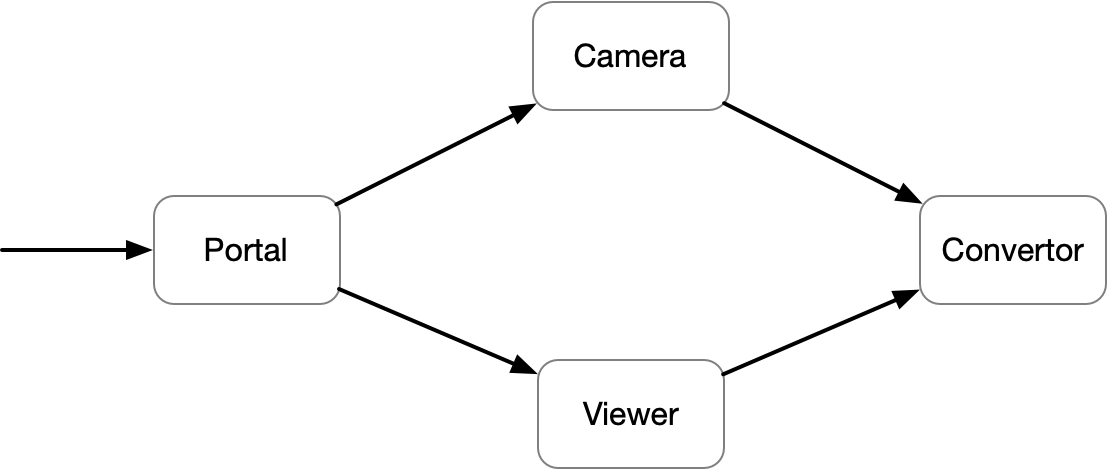
\includegraphics[width= 0.8\textwidth]{image/example.png}
  \caption{示例系统静态依赖图}
  \label{fig:example}
\end{figure}

系统运行的时序图如\ref{fig:timing}。由用户调用在Portal服务上首先开始根事务$T_0$,$T_0$在Camera上发起子事务并得到拍摄数据,为了能够快速传输数据,Camera请求Convertor对数据进行转换,即子事务$T_2$。Camera将得到的内部表示形式的数据返回给Portal。Portal则在Viewer上发起子事务$T_3$,并向其传输数据。Viewer在Convertor上发起新的子事务$T_4$,并将数据进一步传输,最终将解码后的数据结果返回,整个根事务$T_0$结束。

\begin{figure}[!htbp]
  \centering
  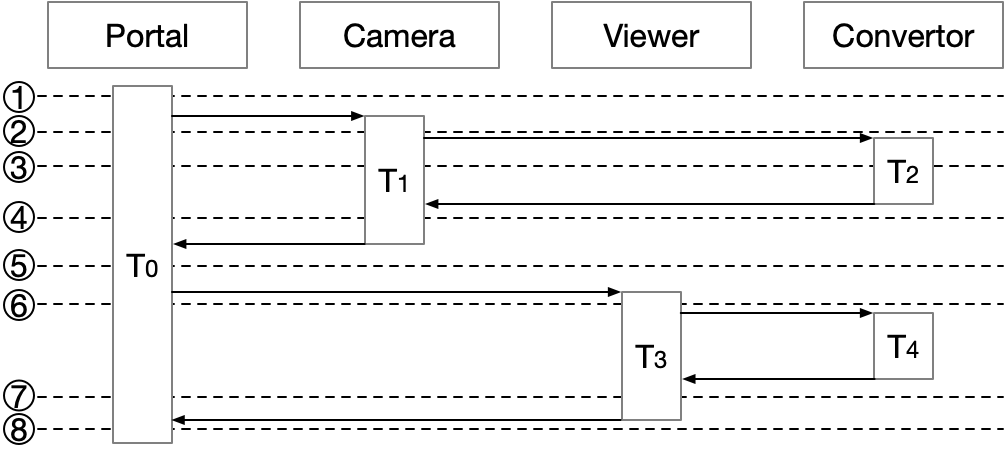
\includegraphics[width= 0.8\textwidth]{image/timing.png}
  \caption{示例系统时序图}
  \label{fig:timing}
\end{figure}

在该软件系统实例中,假设希望提高数据的传输转换速度,系统需要对Convertor服务进行动态更新。若动态更新操作发生在时刻\ding{175}和\ding{177}之间,那么动态更新前的事务由旧版本的Convertor进行编码,而更新完成之后的事务由新版本的Convertor进行解码。若新旧版本的编解码算法不可兼容,便会导致系统出现不一致的情形。因此为满足安全性的需求,动态更新算法需要保证,不存在一个分布式事务的某两个子事务在同一个微服务的不同版本上运行。

\subsection{Quiescence算法}
对于一个分布式系统,通常由若干个节点组成,它们之间相互请求调用从而形成相应的依赖关系。此处节点为泛化代称,在具体的应用场景中,节点有具体的表现形态。当我们需要对此分布式系统中的某个节点执行动态更新操作时,包括节点的创建、删除等,便有可能导致系统的静态依赖关系或目标节点的内部状态发生变化,从而进一步地影响运行时事务的正确性。因此,为了保证动态更新过程中系统的安全性,Kramer和Magee\cite{kramer1990evolving}提出了Quiescence动态更新算法,算法中重点为节点定义了Active和Passive状态:\\

\begin{spacing}{1.0}
\end{spacing}

$\bullet$\textbf{Active}$\indent$处于该状态的节点可以主动地发起事务、接受事务并为其他事务

$\indent\enspace$服务。

\begin{spacing}{2.0}
\end{spacing}

$\bullet$\textbf{Passive}$\indent$处于该状态的节点不能主动地发起新事务,可以继续接受并为其

$\indent\enspace$他事务提供服务,但需要保证:(1)该节点当前不处于自身发起的事务中

$\indent\enspace$(2)该节点不会发起新的事务。 \\

\begin{spacing}{1.0}
\end{spacing}

当某个节点需要执行动态更新操作时,节点的状态可以在Active和Passive之间进行转换,具体的转换关系如图\ref{fig:state_shift}。由前述的Passive状态定义可知,即使节点处于Passive状态下,执行动态更新也不能保证系统的安全性,因为此时节点有可能正在处理由其它节点所发起的事务。因此作者提出了更严格且保证安全性的约束,即Quiescence状态:\\

\begin{spacing}{1.0}
\end{spacing}

$\bullet$$\indent$该节点当前没有参与到自身发起的事务之中

\begin{spacing}{2.0}
\end{spacing}

$\bullet$$\indent$该节点不会发起新的事务

\begin{spacing}{2.0}
\end{spacing}

$\bullet$$\indent$该节点当前未为其他事务提供服务

\begin{spacing}{2.0}
\end{spacing}

$\bullet$$\indent$该节点无需为其他节点已经发起或者是将来会发起的事务服务\\

\begin{spacing}{1.0}
\end{spacing}

\begin{figure}[!htbp]
  \centering
  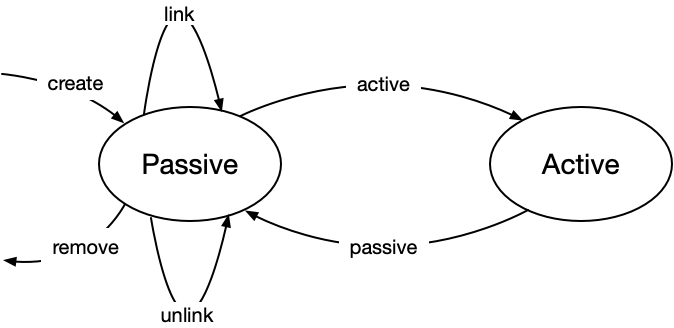
\includegraphics[width= 0.8\textwidth]{image/state_shift.png}
  \caption{Quiescence节点状态转移图}
  \label{fig:state_shift}
\end{figure}

前述对于Quiescence状态的定义中,前两点与Passive状态定义一致,要求当前节点处于Passive状态。而后两点要求本节点不能为其他节点已经发起或者是将来会发起的事务服务,即表示依赖于本节点的其他节点也应处于Passive状态。若某一节点$Q$想要达到Quiescence状态,那么对于集合Passive Set $PS(Q)=\{Q\}\cup\{$直接依赖于$Q$的节点集合$\}$,只有$PS(Q)$中的所有节点均达到Passive状态,节点$Q$才能达到Quiescence状态。

对于$PS(Q)$的定义仅仅考虑了一层依赖关系,更为全面的定义为集合Enlarged Passive Set $EPS(Q)$: \\

\begin{spacing}{1.0}
\end{spacing}

$\bullet$$\indent$$PS(Q)$中的所有节点均属于$EPS(Q)$

\begin{spacing}{2.0}
\end{spacing}

$\bullet$$\indent$所有依赖于$PS(Q)$的节点 \\

\begin{spacing}{1.0}
\end{spacing}

综上,若某一节点$Q$想要达到Quiescence状态,只有当$EPS(Q)$中所有的节点均达到Passive状态时,节点$Q$才能达到Quiescence状态。

在图\ref{fig:example}的示例中,对应的Convertor服务需要等到Portal、Camera、Viewer服务上运行的事务全部结束后才可达到Quiescence状态。可以发现,此时的Portal、Camera、Viewer服务均处于Passive状态,不能发起事务对外提供服务。因此Quiescence算法虽然可以确保动态更新过程中的安全性,但同时给系统带来了极大的干扰\cite{arnold1996software}。

\subsection{Tranquility算法}
Quiescence算法对于安全点的定义过于严格,给运行中的系统带来了极大的干扰。针对此问题,Vandewoude等在Quiescence的基础上提出了Tranquility算法\cite{vandewoude2007tranquility},并利用该算法在DRACO\cite{vandewoude2003draco}中间件上实现了一个动态更新系统。Tranquility算法中继续沿用了Quiescence中事务、Active状态和Passive状态的相关定义,重新为节点定义了Tranquility状态。节点想要达到Tranquility状态需要满足条件:\\

\begin{spacing}{1.0}
\end{spacing}

$\bullet$$\indent$该节点当前没有参与到自身发起的事务中

\begin{spacing}{2.0}
\end{spacing}

$\bullet$$\indent$该节点不会发起新的事务

\begin{spacing}{2.0}
\end{spacing}

$\bullet$$\indent$该节点当前没有处理任何事务

\begin{spacing}{2.0}
\end{spacing}

$\bullet$$\indent$该节点的相邻节点不存在过去使用过此节点并且将来还将使用此节点

$\indent\enspace$的事务。 \\

\begin{spacing}{1.0}
\end{spacing}

在Tranquility的定义中,前两点同样与Passive状态定义一致。而后两点定义均弱于Quiescence的定义,因此满足Quiescence状态的节点必然满足Tranquility状态,但反之则未必。不同点在于,Tranquility算法只要求目标节点处于Passive状态,且与其相邻的节点也处于Passive状态即可。它不需要考虑运行于其它更多节点的事务运行情况,只要相邻的节点不存在使用过目标节点且将来还会使用目标节点的事务,目标节点就可以达到Tranquility状态。

在图\ref{fig:timing}中,当Camera将处理结果返回给Portal后,系统运行到时刻\ding{176},此时Camera、Viewer和Convertor均处于Passive状态,因此Convertor满足Tranquility状态的定义,系统判断可进行更新。但如果此时对Convertor进行版本更新,便有可能因为新版本的Convertor与旧版本存在不可兼容性而出现系统不一致的问题。因此Tranquility算法相比较于Quiescence算法,虽然可以减少对系统造成的干扰,但是无法保证动态更新的过程中系统的安全性问题。

\subsection{Version Consistency算法}
已有的一些动态更新算法或依据静态依赖信息\cite{kramer1990evolving},或依据动态依赖信息\cite{vandewoude2007tranquility,bidan1998dynamic,chen2002component}来保证本地一致性。而马晓星等提出了Version Consistency算法\cite{ma2011version}则对版本一致性的概念进行定义,用于解决了分布式系统下分布式事务的全局一致性问题。

具体来说,Version Consistency中对于一次动态更新可使用如下的元组进行表示:$<\Sigma,\omega,\omega^{'},T,s>$。其中,$\Sigma$表示系统的静态依赖配置,$\omega$表示旧版本的目标集合(即需要动态更新的节点集合),$\omega^{'}$表示新版本的目标节点集合,$T$表示系统状态转移工具,$s$则表示执行动态更新前对应的系统状态。因此,系统执行动态更新后,对应的状态可表示为:$s^{'} = T(s)$。

\begin{definition}[版本一致性]\label{def:VersionConsistency}
对于某一动态更新配置$<\Sigma,\omega,\omega^{'},T,s>$,事务T是满足版本一致性,当且仅当$\nexists T_1,T_2\in ext(T) ~|~ h_{T_1}\in \omega\wedge h_{T_2}\in \omega^{'}$。若当前动态更新配置$\Sigma$中所有的事务都满足版本一致性,那么称此动态更新是版本一致的。
\end{definition}

以图\ref{fig:timing}为示例,系统在时刻\ding{173}之前和时刻\ding{178}之后,对应的$ext(T_0)$中的事务均满足\ref{def:VersionConsistency}的定义,因此都可以进行动态更新。但若系统选择在时刻\ding{176}对Convertor进行动态更新,此时$h_{T_2} = Convertor,h_{T_4} = Convertor^{'}$,且$T_2,T_4 \in ext(T_0)$,显然不满足\ref{def:VersionConsistency}的定义,此次动态更新将使得系统出现版本不一致的情况。

版本一致性虽然定义了动态更新的条件,但该条件在实际应用中需要全局中心化的信息,很难进行操作和检测判断。因此Version Consistency算法使用节点运行时的动态依赖关系,很好地解决了更新状态条件难以判断的问题。在Version Consistency算法中,动态依赖关系由具体的动态依赖边进行定义表示:

\begin{definition}[动态依赖边]\label{def:DynamicDep}
使用$C\xrightarrow[T]{future} C^{'}$表示在根事务T中,节点$C$将来可能会用到节点$C^{'}$;使用$C\xrightarrow[T]{past} C^{'}$表示在根事务T中,节点$C$过去曾经使用过节点$C^{'}$。
\end{definition}

系统在运行时,将依据每一个根事务T的运行状态,动态地在节点间执行依赖边的添加和删除操作。同时要求在对依赖边进行操作的过程中,应满足如下的约束:

\begin{definition}[配置有效性]\label{def:ValidConfig}
使用动态依赖边来表示节点间的动态依赖关系信息是正确有效的,当且仅当对于运行时$future/past$边的创建和删除操作满足以下规则:\\

\begin{spacing}{1.0}
\end{spacing}

$\bullet$$\indent$事务$T$从开始到结束,$T$所在的节点$C$必须存在边$C\xrightarrow[root(T)]{future} C$和$C\xrightarrow[root(T)]{past}$

$\indent$$\enspace$$ C$,其中$root(T)$表示事务$T$的根事务标识;

\begin{spacing}{2.0}
\end{spacing}

$\bullet$$\indent$如果节点$C$和$C^{'}$之间没有相应的静态依赖关系,那么不能建立$C$到$C^{'}$

$\indent$$\enspace$的$future/past$边;

\begin{spacing}{2.0}
\end{spacing}

$\bullet$$\indent$对于边$C\xrightarrow[T]{future} C^{'}$,必须在$ext(T)$的第一个子事务开始前建立,且必须在

$\indent$$\enspace$确定$C$不会再在$C^{'}$上发起子事务后才能够被删除;

\begin{spacing}{2.0}
\end{spacing}

$\bullet$$\indent$对于边$C\xrightarrow[T]{past} C^{'}$,必须在由$C$在$C^{'}$上发起的属于$ext(T)$的子事务结束

$\indent\enspace$之前建立;\\

\begin{spacing}{1.0}
\end{spacing}

\end{definition}

基于动态依赖边,Version Consistency算法提出了Freeness更新判断条件,使得系统只需针对目标更新节点上相关动态依赖边的知识,就可以很方便地判断当前时刻目标更新节点是否满足动态更新的条件。

\begin{definition}[Freeness]\label{def:Freeness}
对于某个配置$\Sigma$,如果当前不存在同时指向节点$C$(或者节点集合$\omega$)的边$C^{'} \xrightarrow[T]{future} C$和边$C^{'} \xrightarrow[T]{past} C$,则称该节点$C$(或者节点集合$\omega$)对根事务$T$是$Freeness$的。若$C$(或者节点集合$\omega$)对于此配置$\Sigma$中的所有事务均是$Freeness$的,则称$C($或者节点集合$\omega$)在配置$\Sigma$中是$Freeness$的。
\end{definition}

图\ref{fig:dyn_dep}展示了系统中某个根事务运行时的动态依赖关系,其中$(a),(b),(c),(d)$分别对应图\ref{fig:timing}中的时刻\ding{172}、时刻\ding{174}、时刻\ding{176}、时刻\ding{178}。利用定义\ref{def:Freeness}可以发现,Convertor在时刻\ding{172}和时刻{178}满足Freeness,不存在标记为$T_0$的一对$future$和$past$边指向Convertor,可进行动态更新;而在时刻\ding{174}和时刻\ding{176}则同时存在标记为$T_0$的$future$和$past$边指向Convertor,因此Convertor不可以进行动态更新。

\begin{figure}[!htbp]
  \centering
  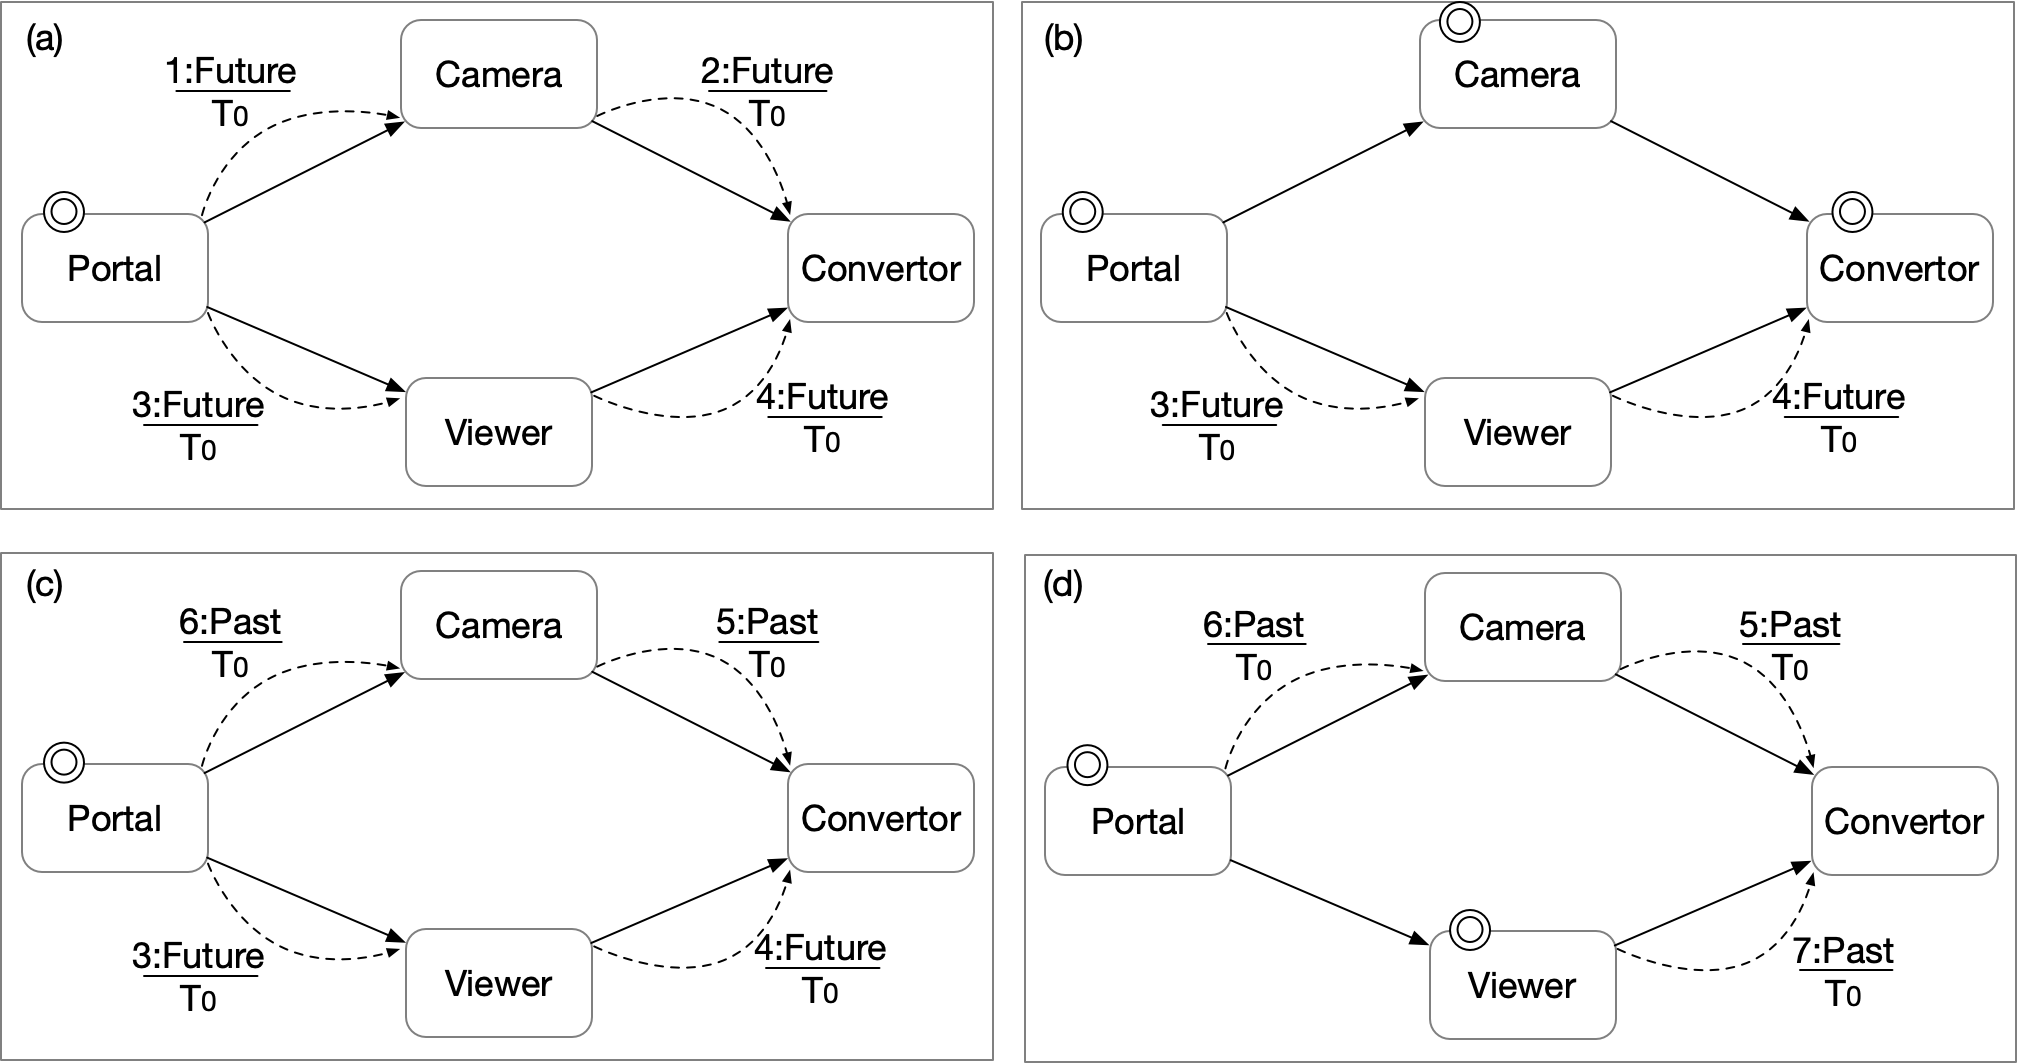
\includegraphics[width= 1.0\textwidth]{image/dyn_dep.png}
  \caption{系统运行时动态依赖关系示例}
  \label{fig:dyn_dep}
\end{figure}

上面介绍的三种具体软件动态更新算法分别对安全更新点给出了自己的定义,即节点分别需要满足Quiescence状态、Tranquility状态和Freeness状态。判断的条件和使用的方式也略有差别,例如Quiescence算法主要利用的是事务和节点间的静态依赖信息,而Version Consistency在其基础上进一步地使用了节点间运行时刻的动态依赖信息,使得对于安全点的判断更为精准。对于前述的动态更新所面临的诸多挑战,如安全性(Safety)、及时性(Timeliness)和干扰性(Disruption),三种算法的表现也不尽相同。具体对比如表\ref{table:comparison}所示。

\begin{table}
  \centering
  \begin{tabular}{ccccp{20mm}}
    \toprule
    \textbf{更新算法} & \textbf{安全性} & \textbf{及时性} & \textbf{干扰性} \\
    \midrule
    Quiescence  & 安全 &  慢  & 高 \\
    Tranquility     & 不安全    &  快  & 低 \\
    Version Consistency     & 安全    &  快  & 低 \\
    \bottomrule
  \end{tabular}
  \caption{动态更新算法比较}
  \label{table:comparison}
\end{table}

\section{微服务架构}
基于微服务理念进行分布式应用程序的开发,已经成为多数平台的通用指导模式\cite{newman2015building,nadareishvili2016microservice}。应用微服务架构的关键之一在于对复杂的业务系统进行拆分,使得拆分出来的服务能够相互保持逻辑上的独立,从而保证服务可由不同的团队进行负责,快速地完成开发、部署和更新等操作。拆分步骤必然导致系统中的模块数量变多,实际上是将原先业务系统内部维护的复杂度,转换成了模块与模块之间的通信与管理监控的复杂度。

随着微服务架构的发展,为了简化开发流程,出现了典型的类库,如Netflix OSS\cite{NetflixOSS}套件,和相关的开发框架,如Spring和Dubbo。框架实现了分布式系统通信的相关通用功能,包括服务发现、负载均衡等,使得开发人员通过编写较少的代码,即可完成分布式微服务系统的开发,有效地提高了开发人员的工作效率。使用相关的开发框架虽然简易,但也存在不少的局限性问题。因此,本节将主要介绍较为主流的微服务框架:Spring、Dubbo,以及处理服务间请求的基础架构层技术:服务网格(Service Mesh)。

\subsection{Spring}
Spring是一个于2003年兴起的轻量级Java开发框架,由Rod Johnson提出,为了解决企业应用开发的复杂而诞生\cite{johnson2004spring}。Spring框架如图\ref{fig:spring_overview}所示,是一种分层架构,共分为如下具体的模块:\\

\begin{figure}[!htbp]
  \centering
  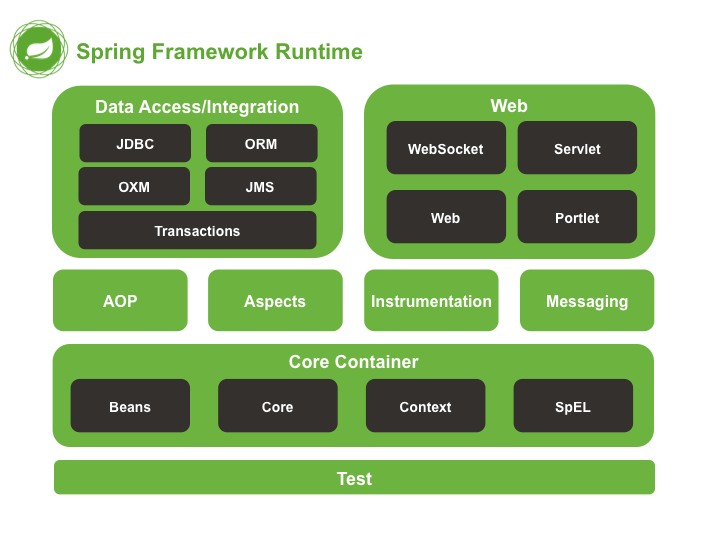
\includegraphics[width= 1.0\textwidth]{image/spring_overview.png}
  \caption{Spring架构图}
  \label{fig:spring_overview}
\end{figure}

\begin{spacing}{1.0}
\end{spacing}

$\bullet$$\indent$\textbf{Core Container}$\indent$核心容器提供Spring的基本功能,使用BeanFactory以控

$\indent$$\enspace$制反转(IOC)的模式来进行依赖注入,以bean的形式组织管理Java程序

$\indent$$\enspace$中的各个组件及其关系。

\begin{spacing}{2.0}
\end{spacing}

$\bullet$$\indent$\textbf{Data Access/Integration}$\indent$提供与多种数据框架集成的相关功能,包括jdbc

$\indent$$\enspace$框架等,实现事务控制的相关模块。

\begin{spacing}{2.0}
\end{spacing}

$\bullet$$\indent$\textbf{Web}$\indent$提供基础的Web集成功能、相关的架构模块和与前端进行双向通信

$\indent$$\enspace$的协议支持。

\begin{spacing}{2.0}
\end{spacing}

$\bullet$$\indent$\textbf{AOP}$\indent$提供多种AOP实现方式的支持,包括AspectJ等。

\begin{spacing}{2.0}
\end{spacing}

$\bullet$$\indent$\textbf{Instrumentation}$\indent$提供了类工具和类加载器的相关实现的支持。

\begin{spacing}{2.0}
\end{spacing}

$\bullet$$\indent$\textbf{Messaging}$\indent$对消息架构和协议的支持。

\begin{spacing}{2.0}
\end{spacing}

$\bullet$$\indent$\textbf{Test}$\indent$提供对单元测试和集成测试的支持。 \\

\begin{spacing}{1.0}
\end{spacing}

分层架构允许开发人员自由地选择需要的组件模块,同时又为J2EE应用程序开发提供完整的集成框架。作为一个较为成熟的开源开发框架,Spring的核心在于控制反转(Inverse of Control, IOC)和面向切面编程(Aspect Oriented Programming, AOP)两部分。其中,控制反转的思想在于利用Spring核心容器进行依赖注入,一方面实现了资源的可配置,另一方面很好地降低了使用资源双方的耦合度;面向切面编程则使得开发人员不修改框架源代码,却能够实现想要的扩展功能,并形成可复用模块。概括来说,Spring的优点主要包括:\\

\begin{spacing}{1.0}
\end{spacing}

$\bullet$$\indent$\textbf{轻量级}$\indent$Spring的体积和管理开销都很小。

\begin{spacing}{2.0}
\end{spacing}

$\bullet$$\indent$\textbf{简化开发}$\indent$将对象间的依赖关系交由Spring控制,降低了业务对象替换时

$\indent$$\enspace$的复杂度,避免硬编码所造成的过度耦合。

\begin{spacing}{2.0}
\end{spacing}

$\bullet$$\indent$\textbf{支持AOP}$\indent$允许将通用任务如日志等进行集中式模块管理。

\begin{spacing}{2.0}
\end{spacing}

$\bullet$$\indent$\textbf{测试}$\indent$可以方便地使用非容器依赖的编程方式来完成测试工作。

\begin{spacing}{2.0}
\end{spacing}

$\bullet$$\indent$\textbf{集成}$\indent$提供了对各种成熟框架的直接支持,降低了开发人员的使用难度。\\

\begin{spacing}{1.0}
\end{spacing}

\subsection{Dubbo}
Dubbo是Alibaba开源的Java分布式服务框架,致力于提供高效的RPC远程服务调用方案以及服务治理方案,被广泛地应用于Alibaba的各方面业务中\cite{ren2014d}。Dubbo的架构与Spring类似,同样属于分层架构,使得各个层之间的耦合度尽量地减少。具体的服务调用关系流程如图\ref{fig:dubbo_overview}所示:\\

\begin{figure}[!htbp]
  \centering
  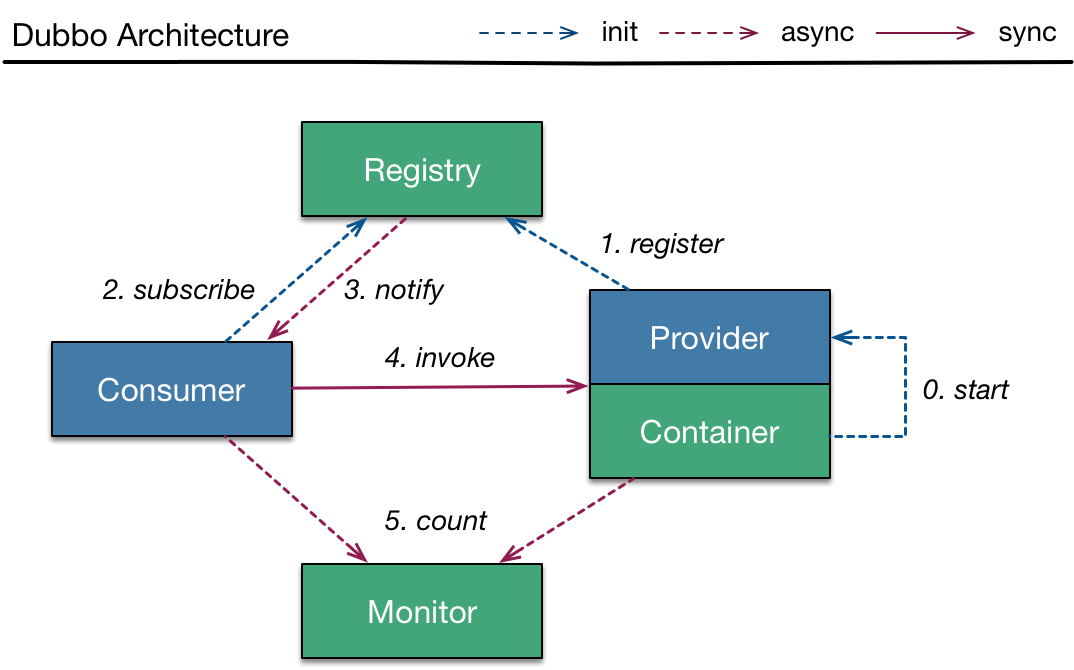
\includegraphics[width= 1.0\textwidth]{image/dubbo_overview.png}
  \caption{Dubbo服务调用关系图}
  \label{fig:dubbo_overview}
\end{figure}

\begin{spacing}{1.0}
\end{spacing}

$\bullet$$\indent$服务提供方运行容器并向注册中心进行注册;

\begin{spacing}{2.0}
\end{spacing}

$\bullet$$\indent$服务调用方向注册中心进行订阅,获取服务提供方的地址信息并进行

$\indent$$\enspace$调用;

\begin{spacing}{2.0}
\end{spacing}

$\bullet$$\indent$Monitor监控模块负责异步地接收调用过程中的相关信息。 \\

\begin{spacing}{1.0}
\end{spacing}

Dubbo主要提供了服务注册和服务调用的相关功能,服务注册方面使用的自动注册和管理机制,使得服务调用方不需要硬编码服务方地址,提供多种注册中心的选择。服务调用方面透明化远程方法的调用,自动为服务调用方提供软负载均衡及容错机制。Dubbo架构具有连通性、健壮性和伸缩性等特点,有助于增强服务治理,使得传统的单体应用程序可以逐步平滑地重构为可扩展的分布式微服务架构。

\subsection{Service Mesh}
虽然开发框架本身对用户屏蔽了绝大多数通用功能的实现细节,但开发人员同样需要耗费大量时间与精力去学习掌握框架本身。同时,开发框架通常局限于一种或几种特定的编程语言,业务服务往往得随着框架服务的升级而升级。

Mogan于2017年在其文章中提出Service Mesh的概念\cite{morgan2017sa}。Service Mesh考虑使用边车模式(Sidecar),为每一个服务实例部署一个对应的Sidecar实例,开发人员只需关注核心的业务逻辑代码,而由Sidecar实例来负责实现服务发现、负载均衡、认证授权等通用性功能\cite{li2019service,el2019guiding}。Service Mesh的架构图如图\ref{fig:service_mesh}所示:

\begin{figure}[!htbp]
  \centering
  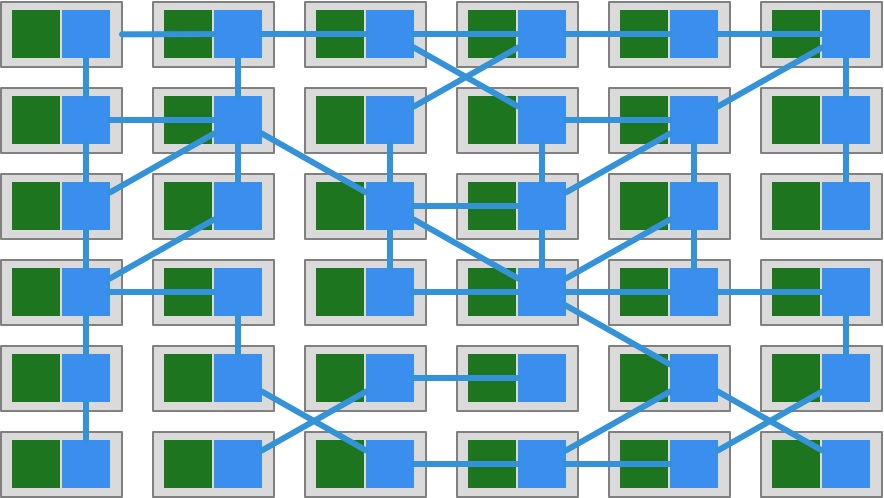
\includegraphics[width= 0.8\textwidth]{image/service_mesh.png}
  \caption{Service Mesh架构}
  \label{fig:service_mesh}
\end{figure}

随着微服务数量的增加,部署的Sidecar实例也逐渐增加,服务与Sidecar、Sidecar之间的通信便形成了一个错综复杂的网络,也即是服务网格(Service Mesh)名称的由来。Service Mesh插入的Sidecar实例通常为轻量级的网络代理,资源占用消耗较小,对部署的服务实例保持透明性。此外,Service Mesh将原本通过开发框架实现的通用性功能,从应用服务代码中解耦出来,降低耦合度的同时也可保证Service Mesh的组件可以独立于业务服务单独升级。

\subsection{微服务架构与动态更新}
随着微服务架构的流行,相关动态更新的工作也有了较多的关注,目前已经出现了不少的研究成果。

在Spring框架中,支持两种热部署(Hot Deploy)的方式,热部署主要希望在修改应用代码时,不重启停止应用即可完成代码的更新。此功能类似与动态更新(动态配置),但是在具体的实现上,热部署主要基于Java的动态类加载机制,不能很好地定义安全点,无法保证应用更新过程中的正确性和一致性。例如在Spring框架中,Spring Load是一个用于在JVM运行时重新加载类文件更改的JVM代理,允许用户动态对某个方法字段等进行添加、修改、删除。当使用Spring Load启动程序后,系统会自动监视对应的文件,当目标文件发生改动时,系统便会重新加载类文件,无需重启服务。Devtools的功能类似,原理在于使用两个类加载器:不改变的类包括第三方jar,由base类加载器加载,而目标正在开发的类由restart类加载器加载。当检查到类发现变化时,应用进行重启,restart类加载器直接丢弃重建,而base类加载器则继续留用。由于base类加载器已经可用且已填充,因此本次应用的重启会比普通的重启速度要快得多。这两种热部署的实现方式均考虑的是目标文件的相关变化,但并不关心更新过程中运行时事务的相关状态,因此无法保证更新的正确性。

微服务架构具有耦合度低、独立部署扩展等特性,因此它通常在相关的分布式云服务平台上进行部署运行并使用其底层框架的能力\cite{sampaio2017supporting}。例如Spinnaker\footnote{Spinnaker. https://www.spinnaker.io/}, AWS CodeDeploy\footnote{AWS CodeDeploy. https://aws.amazon.com/codedeploy/}, IBM UrbanCode\footnote{IBM UrbanCode. https://developer.ibm.com/urbancode/}都支持对部署于异构Paas平台上的微服务进行更新部署。更新的执行主要依靠运维人员对底层操作进行编写,并形成一系列的流水线操作,最后以脚本的形式来运行。这种更新方法具有较大的局限性,一方面它要求运维人员撰写出正确且有效的运行脚本,这通常需要耗费较长的调试时间;另一方面,脚本的执行通常不具有幂等性,如果基于脚本的更新过程出现异常的话,往往需要回滚并重启整个更新过程,并小心翼翼地保存相关的状态。push2cloud\footnote{Push2Cloud website. https://push2.cloud/}则运行对更新的目标系统结构进行描述,并支持部署在其上的微服务进行更新。但目前仅支持单站点的微服务部署,更新策略同样需要定义成对应平台的底层流水线操作。

\section{本章小结}
本章主要介绍了软件动态更新的相关算法,以及现有主流的微服务框架、相关微服务架构对动态更新方面的支持。在软件动态更新的相关算法中,本章重点介绍了Quiescence、Tranquility和Version Consistency三种算法,它们分别在各自的算法中对动态更新的安全点进行定义,以及安全点的相关判断条件。同时还对这三种算法在安全性(Safety)、及时性(Timeliness)和干扰性(Disruption)进行了具体的比较。而在现有主流的微服务框架中,主要介绍了Spring、Dubbo框架,以及新一代的Service Mesh技术,对其架构和相关特性进行了说明。最后介绍了Spring框架对于热部署机制的两种支持方式,以及相关分布式云服务平台对微服务架构在动态更新方面的支持。

%%%%%%%%%%%%%%%%%%%%%%%%%%%%%%%%%%%%%%%%%%%%%%%%%%%%%%%%%%%%%%%%%%%%%%%%%%%%%%%
\chapter{支持事务一致性的微服务动态更新方法}\label{chapter_3}
动态更新在实际应用场景中有着较大的需求,但当前的微服务架构对更新过程中的安全性考虑不足,缺乏对服务正确且快速更新的支持。本章首先对微服务动态更新的挑战进行讨论,分析当前的微服务架构在动态更新支撑方面的不足。然后基于上述讨论与分析,针对性地在事务模型、动态依赖管理和服务生命周期三个方面提出了相应的扩展和实现方案,并选择在服务网格Service Mesh之上进行相关模型的扩展,给出一种支持事务一致性的微服务动态更新实现方法VCIM(Version Consistency In Microservices)。

\section{需求与挑战}
为了在微服务架构之上,支持相关的动态更新算法,我们需要考虑:\\

\begin{spacing}{1.0}
\end{spacing}

$\bullet$$\indent$\textbf{事务模型}

$\indent$$\enspace$前述动态更新算法中均与事务模型相关,依据前述对于事务的定义\ref{def:transaction},

$\indent$$\enspace$是指服务上执行的一系列有意义的动作。而当前相关的微服务框架所支

$\indent$$\enspace$持的事务主要指传统数据库中的ACID(Atomicity, Consistency, Isolation,

$\indent$$\enspace$ Durability)事务,如Spring框架中的@Transactional注解,无法为更新

$\indent$$\enspace$算法中的事务提供有效的语义支持。事务是服务运行时处理请求的基础

$\indent$$\enspace$,事务的状态一定程度上反映当前服务所处的状态,是动态更新算法判

$\indent$$\enspace$断系统状态的重要依据。因此,我们需要为微服务系统定义合适的事务

$\indent$$\enspace$状态模型,为更新算法提供运行时事务信息。

\begin{spacing}{2.0}
\end{spacing}

$\bullet$$\indent$\textbf{动态依赖管理}

$\indent$$\enspace$服务间的静态依赖关系可以保守地对系统运行时进行描述,但是无法保

$\indent$$\enspace$证动态更新的及时性。基于运行时服务间的动态依赖信息,动态更新算

$\indent$$\enspace$法可以有效地对安全更新点进行判断,在保证动态更新一致性的前提下

$\indent$$\enspace$,及时地完成服务的更新。因此,我们需要维护服务间的动态依赖信息

$\indent$$\enspace$,为更新算法提供基础保障。

\begin{spacing}{2.0}
\end{spacing}

$\bullet$$\indent$\textbf{服务生命周期}

$\indent$$\enspace$现有的微服务系统通常仅考虑服务的基本状态,包括初始状态、运行状

$\indent$$\enspace$态、终止状态等。显然单一的运行状态并不能很好地刻画目标服务在整

$\indent$$\enspace$个更新过程中的状态。具体来说,除了相关的基本状态,运行状态的服

$\indent$$\enspace$务从收到更新请求到最后更新结束,还需包括更多拥有特定意义的状态

$\indent$$\enspace$,如更新开始状态、版本切换状态、结束撤销状态等。因此,我们需要

$\indent$$\enspace$对更细粒度的服务生命周期及其状态跳转进行定义,保证更新前后的一

$\indent$$\enspace$致性和持续性。 \\

\begin{spacing}{1.0}
\end{spacing}

与此同时,支持动态更新的微服务架构还面临着不少挑战。该架构还需尽量保证:\\

\begin{spacing}{1.0}
\end{spacing}

$\bullet$$\indent$动态更新开始前,用户可以对目标更新服务进行指定,且更新前后需保

$\indent$$\enspace$证系统的安全性(定义\ref{def:safety}),不会出现因更新而导致的不一致现象。

\begin{spacing}{2.0}
\end{spacing}

$\bullet$$\indent$能够尽快地完成动态更新,有较好的及时性,且更新过程不会对整个系

$\indent$$\enspace$统,包括其它非更新服务带来较大的干扰,保持良好的用户体验。

\begin{spacing}{2.0}
\end{spacing}

$\bullet$$\indent$内部的相关模块具有较低的耦合度,从而保证不会对基于此架构开发的

$\indent$$\enspace$应用造成较大的影响,可以适配实际不同应用场景下的微服务系统,具

$\indent$$\enspace$有较好的兼容性。\\

\begin{spacing}{1.0}
\end{spacing}

基于上述的讨论和分析,为使当前的微服务系统支撑具体的动态更新算法,我们需要对事务模型、动态依赖管理、服务生命周期等进行扩展实现,并将其整合到相应的微服务架构中。

\section{支持微服务动态更新的方法}
实际应用场景下,不同的微服务系统将由不同的团队来进行开发,在通信方式、编程语言、运行环境等方面都存在较大的差异。而上述讨论均是针对微服务系统中将要扩展的模块来进行,与具体的微服务业务逻辑无关,应保证两者之间的松耦合性。因此,我们选择Service Mesh支撑微服务的底层架构,在其上进行相关模块的实现扩展和整合,给出一种支持事务一致性的微服务动态更新实现方法VCIM(Version Consistency In Microservices)。

使用Service Mesh作为微服务的底层实现架构的优势主要体现在:\\

\begin{spacing}{1.0}
\end{spacing}

$\bullet$$\indent$Service Mesh使用流量代理的方式来对具体的微服务实例进行管理,因此

$\indent$$\enspace$相关的扩展模块可以使用相同的方式来进行实现,在保证透明性的同时

$\indent$$\enspace$,开发人员的业务代码具有较小的侵入性。

\begin{spacing}{2.0}
\end{spacing}

$\bullet$$\indent$Service Mesh允许开发人员选择自身偏好的编码语言,只需保证微服务间

$\indent$$\enspace$的网络可达性即可,可适配于实际应用场景下不同类型的微服务系统。

\begin{spacing}{2.0}
\end{spacing}

$\bullet$$\indent$Service Mesh架构可保证微服务与动态更新的管理模块解耦开,两者都可

$\indent$$\enspace$独立地完成升级。

\begin{spacing}{1.0}
\end{spacing}

\subsection{事务模型与依赖管理}
运行时事务信息和服务间的动态依赖信息是更新算法判断服务能否被更新的基础依据。动态依赖信息需要同特定的事务相绑定才有具体的表征意义,因此VCIM扩展实现了事务依赖管理器,统一负责对运行时事务和动态依赖进行管理。

VCIM首先对事务的状态进行了定义,如图\ref{fig:transaction_shift}所示。具体来说,相关的状态包括:初始化、运行、依赖变更、结束。\\

\begin{spacing}{1.0}
\end{spacing}

$\bullet$$\indent$\textbf{初始化}~当服务接收到外来请求并被流量代理所拦截时,生成相应的事务

$\indent$$\enspace$,且事务进入初始化状态。此时的事务还未被真正的服务实例处理,请

$\indent$$\enspace$求将被进一步地转发。

\begin{spacing}{2.0}
\end{spacing}

$\bullet$$\indent$\textbf{运行}~当服务实例开始执行由流量代理转发而来的事务时,事务进入运行

$\indent$$\enspace$状态,表示事务开始执行具体的业务逻辑。

\begin{spacing}{2.0}
\end{spacing}

$\bullet$$\indent$\textbf{依赖变更}~事务在运行时有可能对一个或多个依赖服务发起远程调用,并

$\indent$$\enspace$在其之上发起相应的子事务。当远程调用返回时,服务间的动态依赖关

$\indent$$\enspace$系便可能发生变化,当前服务已经使用过该依赖服务,以及当前服务在

$\indent$$\enspace$将来是否还会调用该依赖服务。处于依赖变更状态的事务仍处于运行状

$\indent$$\enspace$态,若后续还存在相关的远程调用,则此事务状态保持不变,否则,等

$\indent$$\enspace$待事务执行完成,将转入结束状态。

\begin{spacing}{2.0}
\end{spacing}

$\bullet$$\indent$\textbf{结束}~当事务执行完成时,将结果经流量代理返回给具体的调用者。此时

$\indent$$\enspace$事务进入结束状态,表示一次事务完整的执行。 \\

\begin{spacing}{1.0}
\end{spacing}

\begin{figure}[!htbp]
  \centering
  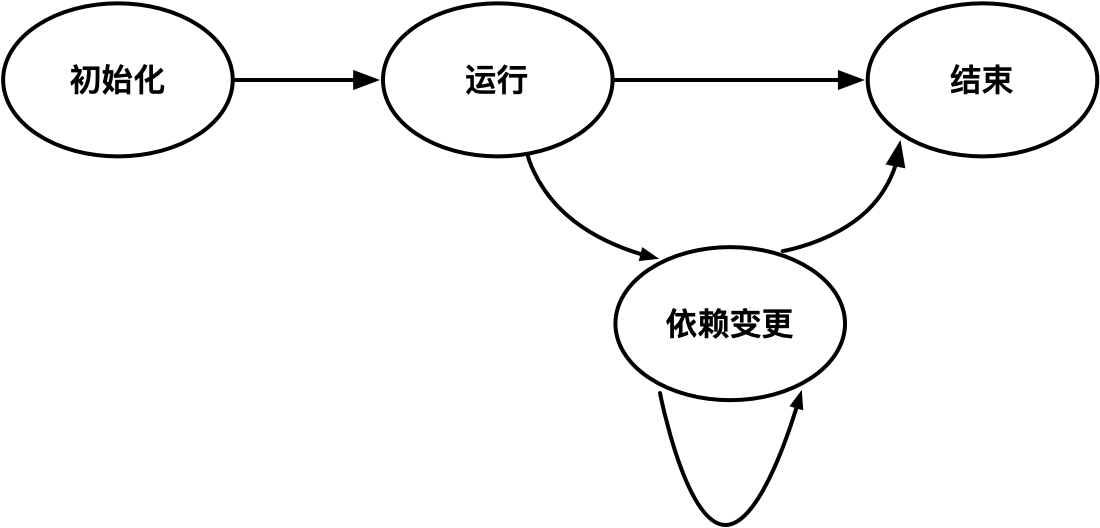
\includegraphics[width= 0.8\textwidth]{image/transaction_shift.png}
  \caption{事务状态转移图}
  \label{fig:transaction_shift}
\end{figure}

分布式事务状态的定义与事务状态的定义保持一致,不同之处在于它由其所有的子事务的状态来共同表示。这些子事务的状态在分布式服务实例的本地进行维护,不存在中心化的存储。当系统在需要相关信息时,每个服务可借助于分布式事务标识信息,向依赖于自己的相关服务发起请求,获得全局的分布式事务信息状态。

事务运行时状态影响服务间的动态依赖关系,反之服务间的动态依赖关系也需要具体的事务来进行标识,两者密切相关,相互耦合。VCIM通过对具体的程序进行分析,得到相对应的事务状态自动机,并利用此事务状态机来进行动态依赖信息的获取\cite{su2013automated}。当本地事务运行时,事务的依赖会发生相应的变化,从而反映出服务间依赖关系的变化。该事务状态自动机将分析出在当前状态下,事务曾经调用过的服务集合PAST\_SET,以及将来有可能需要调用的服务集合FUTURE\_SET,依据此信息形成动态依赖关系,并在本地进行管理。

虽然VCIM从服务启动后就在不断地维护相关的事务和动态依赖信息,但可以看到VCIM对事务模型的定义较为精简,每个服务只需知晓和维护其本地事务的详细信息和对应的分布式事务标识,而无需在服务间进行事务上下文的同步工作,尽可能地减少对全局事务信息的维护,从而避免了服务间通信所带来的额外开销,并且达到了对相关模块减负的目的。

\subsection{服务生命周期}
Service Mesh架构并未对运行于之上的服务的生命周期进行相关的约束,VCIM需要对系统中服务的生命周期模型进行更细粒度的扩展定义。该生命周期模型应包括动态更新过程中以及结束后服务可能的状态,以及状态间如何完成跳转,形成一次完整的更新闭环流程,为系统提供多次连续更新的能力。因此,如何对生命周期模型进行合适的定义,是服务正确进行动态更新的关键因素。本节将对动态更新过程中,服务的生命周期模型进行具体的定义,包括相关的服务状态及跳转关系。

VCIM允许用户在执行动态更新前指定需要更新的服务,称为目标更新服务,该服务可能对应于多个具体的服务实例。此处扩展的服务生命周期模型主要是针对于服务运行时(Running)状态的扩展,这里服务的状态将代表系统对外暴露的服务运行情况,是所有服务实例运行状态的总称,而不是特指某一个服务实例的运行状态。扩展后的服务生命周期模型如图\ref{fig:svc_lifecycle}所示,具体包括了:\\

\begin{spacing}{1.0}
\end{spacing}

$\bullet$$\indent$\textbf{Normal}~当服务初始启动就绪,或者某次更新完成后,服务将进入Normal

$\indent$$\enspace$状态。处于Normal状态下的服务和未扩展前正常运行状态下的服务一

$\indent$$\enspace$致,系统仅存在(使用)一个版本的服务实例来处理外来请求。

\begin{spacing}{2.0}
\end{spacing}

$\bullet$$\indent$\textbf{Deployed}~当用户想要对某个服务进行动态更新时,首先需要上线相应的

$\indent$$\enspace$新版本服务实例并等待其全部就绪,此时服务进入Deployed状态。此时

$\indent$$\enspace$系统中对应的服务包括新旧多个版本实例,但请求仅由旧版本的服务实

$\indent$$\enspace$例来进行处理。若此时未能确保所有新版本服务实例就绪,则后续随着

$\indent$$\enspace$服务状态的转变,将请求发往未就绪的实例时,便会导致异常,返回错

$\indent$$\enspace$误结果。

\begin{spacing}{2.0}
\end{spacing}

$\bullet$$\indent$\textbf{Prepared}~服务在完成Deployed状态之后,用户可指定目标更新服务,并

$\indent$$\enspace$向系统发送动态更新请求。如何正确地为用户请求选择合适的服务实例

$\indent$$\enspace$,取决于流量代理模块中的相关配置。为了能够保证流量在新旧版本的

$\indent$$\enspace$服务实例间进行切换,VCIM首先需要对相关服务的流量代理模块添加相

$\indent$$\enspace$关的路由规则,完成更新的准备工作,服务进入Prepared状态。

\begin{spacing}{2.0}
\end{spacing}

$\bullet$$\indent$\textbf{Shifted}~当前述动态更新的准备工作完成后,VCIM更新相关服务的流量

$\indent$$\enspace$代理模块中的相关路由规则,进行流量的切换,服务进入Shifted状态。

$\indent$$\enspace$当存在外来请求向目标更新服务发起调用时,若该请求对应的分布式事

$\indent$$\enspace$务曾经在目标更新服务上发起过子事务,那么请求将被转发往旧版本的

$\indent$$\enspace$服务实例;否则,请求将被转发往新版本的服务实例。显然,处于此状

$\indent$$\enspace$态中的服务对于用户请求的处理满足定义\ref{def:safety}中对于动态更新的安全性

$\indent$$\enspace$要求。

\begin{spacing}{2.0}
\end{spacing}

$\bullet$$\indent$\textbf{Freeing}~为了避免旧版本服务实例对于系统资源持续占有所造成的浪费,

$\indent$$\enspace$用户向目标更新服务发起撤销旧版本的请求,服务进入Freeing状态。在

$\indent$$\enspace$此状态下,目标更新服务将向依赖于自己的相关服务发起请求,并获得

$\indent$$\enspace$相关的事务和动态依赖信息。同时结合本地所维护的相关信息,若所有

$\indent$$\enspace$在目标更新服务上发起过子事务的分布式事务均不会再次向目标更新服

$\indent$$\enspace$务发起请求,同时目标更新服务的所有旧版本服务实例当前都没有在执

$\indent$$\enspace$行事务。则目标更新务满足定义\ref{def:Freeness}中的Freeness条件,旧版本服务实

$\indent$$\enspace$例可以被正确撤销。

\begin{spacing}{2.0}
\end{spacing}

$\bullet$$\indent$\textbf{Updated}~处于Freeing状态的服务在满足Freeness条件后,便可执行旧版

$\indent$$\enspace$本实例的撤销操作,服务进入到Updated状态。在此状态下,VCIM将对

$\indent$$\enspace$相关服务的流量代理模块进行路由规则的重配置和相关事务的标记清理

$\indent$$\enspace$工作。目标更新服务完成更新,回到Normal状态,完成一次完整的动态

$\indent$$\enspace$更新闭环流程。\\

\begin{spacing}{1.0}
\end{spacing}

\begin{figure}[!htbp]
  \centering
  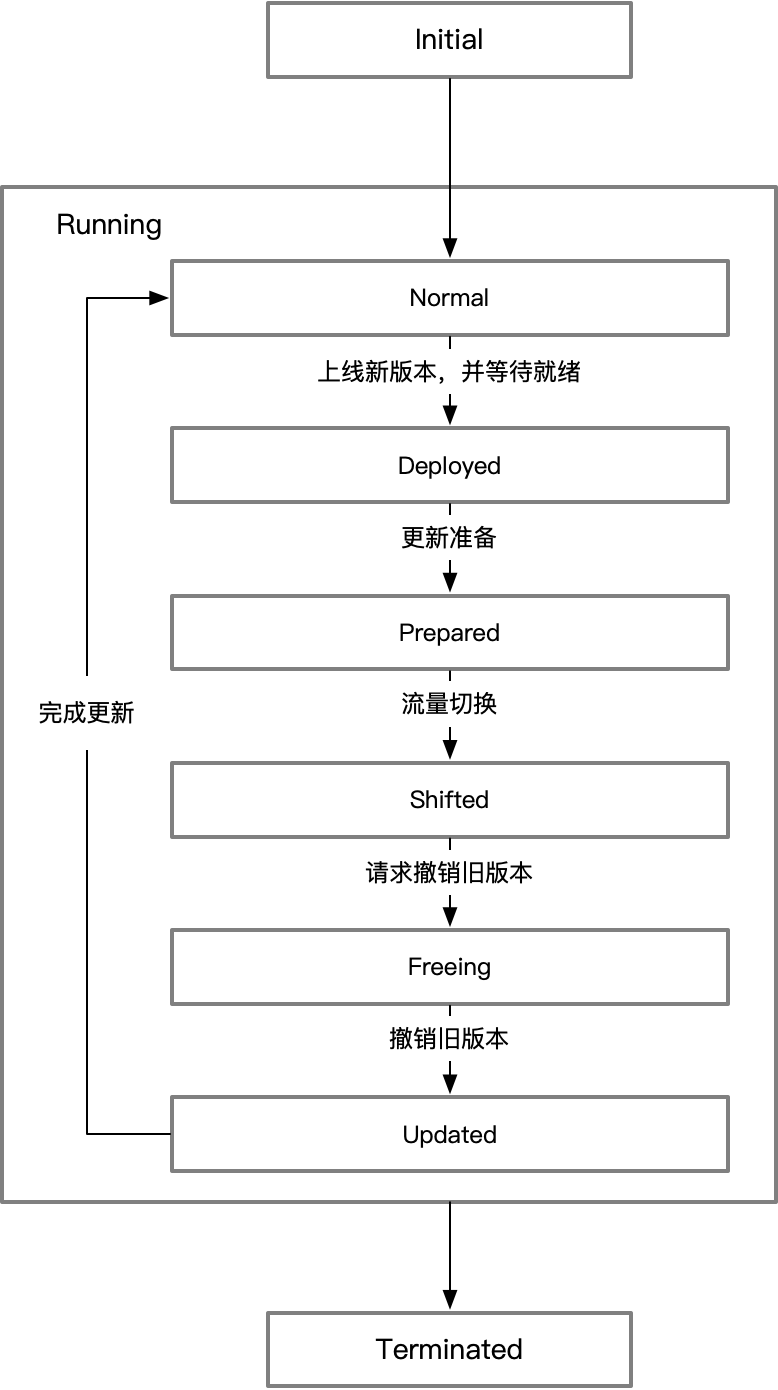
\includegraphics[width= 0.6\textwidth]{image/svc_lifecycle.png}
  \caption{服务生命周期}
  \label{fig:svc_lifecycle}
\end{figure}

在前述动态更新的过程中,VCIM仅关注目标更新服务的状态变化情况。在特定状态下,目标更新服务需要向依赖于自身的相关服务发起请求,以获得动态依赖信息,但并不对相关服务的状态进行限定。这意味着使用VCIM方法扩展的服务生命周期模型具有较好的隔离性,将不同服务间的状态解耦开,有效地提高了更新的效率。

由于普通的微服务通常具有无状态、即插即用等特性,因此其生命周期较为简单,无法对动态更新中的相关语义进行理解。VCIM通过对服务的生命周期模型进行扩展,很好地满足了动态更新过程中对于目标服务不同阶段的更新状态的需求。此外,动态更新中具体的版本更新切换算法和旧版本撤销算法,可在生命周期模型中的相应状态中进行具体的实现。

\section{本章小结}
本章主要对支持事务一致性的微服务动态更新方法VCIM进行了介绍。首先,对当前微服务架构支持动态更新所面临的挑战进行了探讨,对其不足和需求进行了具体的分析。然后针对相应的问题,有效地在事务模型、动态依赖管理和服务生命周期三个方面提出了具体的扩展方案。基于上述模型在Service Mesh上的扩展,给出对应的实现方法VCIM。下一章将结合具体的微服务系统示例,对VCIM的具体系统实现进行详细的阐述和说明。

%%%%%%%%%%%%%%%%%%%%%%%%%%%%%%%%%%%%%%%%%%%%%%%%%%%%%%%%%%%%%%%%%%%%%%%%%%%%%%%
\chapter{支持动态更新的微服务系统实现}\label{chapter_4}
在上一章中,VCIM具体从事务模型、动态依赖管理和服务生命周期三个方面,对支持动态更新的微服务架构进行了扩展。本章将根据第三章中提出的VCIM方法,结合具体的微服务系统示例,介绍如何在开源框架Istio之上进行具体设计,实现支持动态更新算法的微服务系统。

\section{系统设计概述}
根据章节\ref{chapter_3}中的介绍,为使Service Mesh架构支持服务的动态更新,这里考虑使用与流量代理类似的方式,对事务和依赖管理进行扩展。同时,为了使用户可以方便地对系统执行动态更新等操作,在具体的应用系统之外,定义了额外的服务生命周期模型和更新控制模块,为应用系统提供相应的管理功能,实现了模块间耦合度的降低。

概括来说,支持动态更新的微服务系统设计目标和准则包括:\\

\begin{spacing}{1.0}
\end{spacing}

$\bullet$$\indent$兼容当前Service Mesh以及微服务的相关标准。在完成动态更新功能的支

$\indent$$\enspace$持后,对任何正常开发部署的微服务应用都不应造成影响。

\begin{spacing}{2.0}
\end{spacing}

$\bullet$$\indent$添加的相关模块应保证动态更新过程的安全性、及时性和低干扰性。即

$\indent$$\enspace$要求动态更新过程可以高效的完成,同时不会对系统中正常业务的请求

$\indent$$\enspace$造成干扰,破坏系统的一致性。

\begin{spacing}{2.0}
\end{spacing}

$\bullet$$\indent$提供相应的动态更新管理接口,允许用户对系统中服务状态进行查询,

$\indent$$\enspace$和发起动态更新请求等操作,系统依据服务的相关状态,自动完成动

$\indent$$\enspace$态更新操作。 \\
\begin{spacing}{1.0}
\end{spacing}

\section{系统扩展实现}
本节将基于上一章提出的扩展方案,对相关的扩展模块进行实现,并且为用户提供相关的动态更新管理接口。下面将详细阐述事务依赖管理器模块$TxDepManager$、服务生命周期管理器模块$SvcLifecycleManager$,以及更新控制模块$UpdateController$的内部结构设计。

\subsection{事务依赖管理器}
为了使微服务系统能够对运行时事务提供相关的语义支持,维护服务间的动态依赖关系,定义了事务依赖管理器模块,并选择Service Mesh作为支撑微服务的底层实现架构。当前主流的Service Mesh实现方案是Google、IBM及Lyft合作开发的Istio开源框架\cite{sheikh2018modernize,wang2019developing}。Service Mesh架构为每一个微服务实例均部署特定的网络代理,整个系统引入了大量独立运行的单机代理服务。为了更好地保障系统的整体稳定性,Istio使用集中式的控制面板,提供了统一的管理运维入口,具体架构图如图\ref{fig:istio_arch}所示,其中:\\

\begin{spacing}{1.0}
\end{spacing}

$\bullet$$\indent$\textbf{控制平面(Control Plane)}~负责监听底层平台数据源,作为配置中心,将

$\indent$$\enspace$实时的配置信息动态地发往数据平面,控制整个系统的通信等各方面行

$\indent$$\enspace$为;

\begin{spacing}{2.0}
\end{spacing}

$\bullet$$\indent$\textbf{数据平面(Data Plane)}~自动注入的所有服务实例的流量代理总称,负责连

$\indent$$\enspace$接到控制平面并接收相关配置信息,然后对请求按配置进行处理,是配

$\indent$$\enspace$置规则的实际执行者; \\

\begin{spacing}{1.0}
\end{spacing}

\begin{figure}[!htbp]
  \centering
  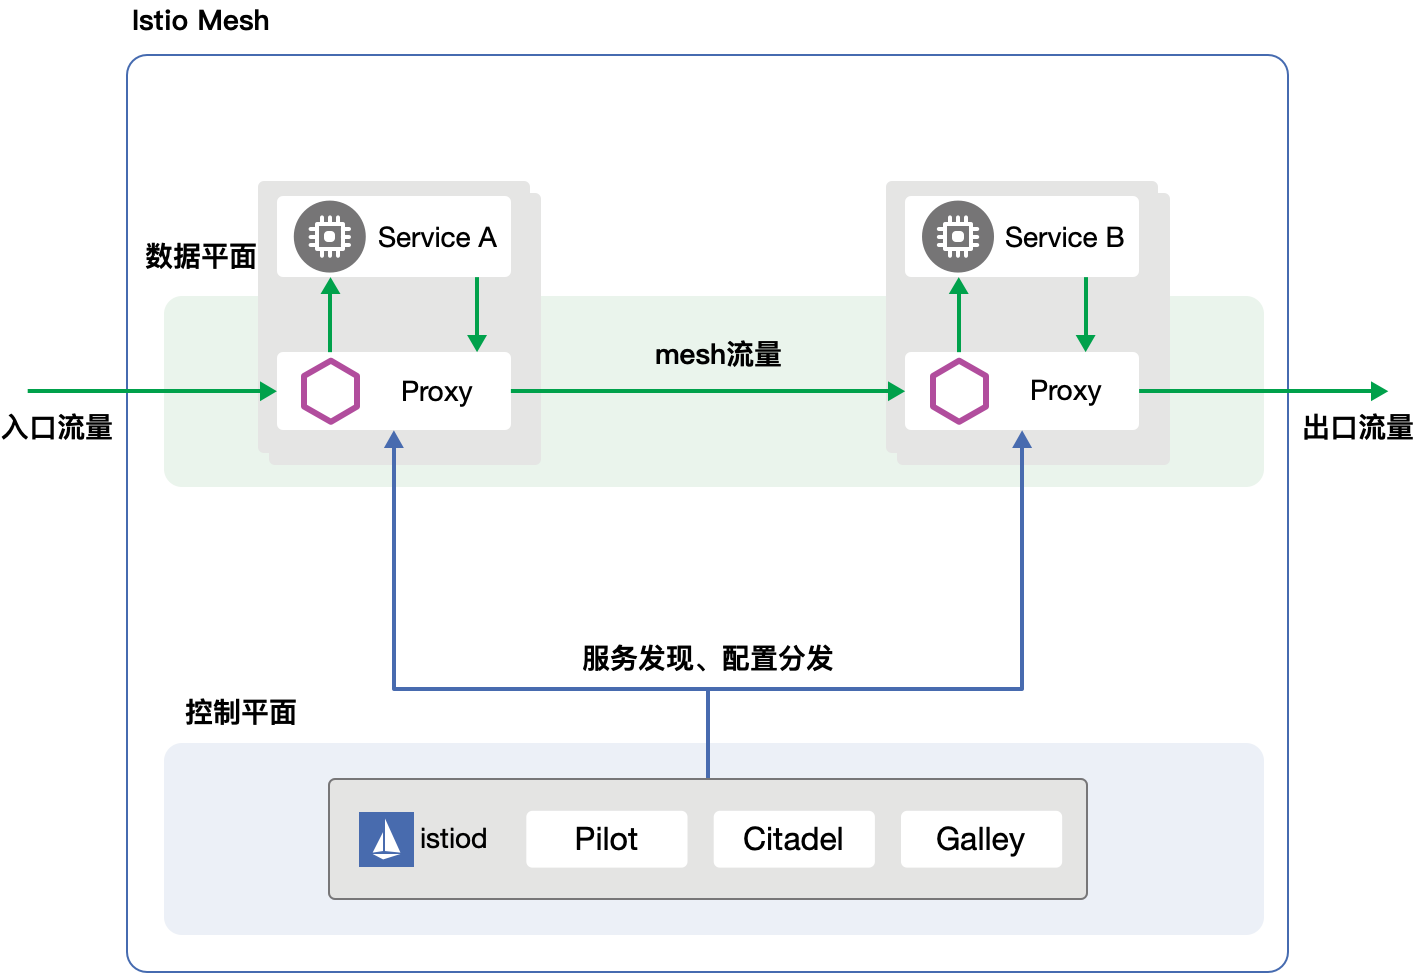
\includegraphics[width= 1.0\textwidth]{image/istio_arch.png}
  \caption{Istio架构图}
  \label{fig:istio_arch}
\end{figure}

为实现VCIM中对于事务与依赖的扩展模型,我们选择在数据平面对相关模型提供支持。扩展后的某个具体的微服务实例如图\ref{fig:instance_model}所示,其中包括了:\\

\begin{spacing}{1.0}
\end{spacing}

$\bullet$$\indent$\textbf{流量代理}~拦截并接管所有的外来请求,生成相应的本地事务并添加或继

$\indent$$\enspace$承特定的分布式事务标识。流量代理模块一方面负责将请求分发至相应

$\indent$$\enspace$的业务逻辑模块,另一方面负责对前述的事务上下文信息进行传递。

\begin{spacing}{2.0}
\end{spacing}

$\bullet$$\indent$\textbf{事务依赖管理器}~负责事务与依赖的管理,保证在事务依赖发生变更时,

$\indent$$\enspace$对相应的服务集合PAST\_SET和FUTURE\_SET等信息进行更新保存,

$\indent$$\enspace$为VCIM提供运行时事务信息和动态依赖信息。

\begin{spacing}{2.0}
\end{spacing}

$\bullet$$\indent$\textbf{业务逻辑}~由服务的开发人员完成编写,从流量代理模块接收请求,执行

$\indent$$\enspace$真正的业务逻辑并返回结果,再由流量代理模块将结果进一步地返回给

$\indent$$\enspace$调用者。\\

\begin{spacing}{1.0}
\end{spacing}

其中,流量代理模块和事务依赖管理器通过UDS\footnote{https://en.wikipedia.org/wiki/Unix\_domain\_socket}(Unix Domain Socket)进行通信,UDS通过指定同一主机上的socket文件,不需要经过网络协议栈即可完成数据的传输,效率较高。同时相关的数据总是以单向的形式发送,因此不会对流量代理模块中的请求处理分发流程造成阻塞,保证了对系统具有较低的干扰性。与此同时,流量代理模块对业务逻辑保持透明,为其屏蔽了调用方的相关细节,开发人员只需关注于业务代码,可以很好地与其它模块解耦开。

\begin{figure}[!htbp]
  \centering
  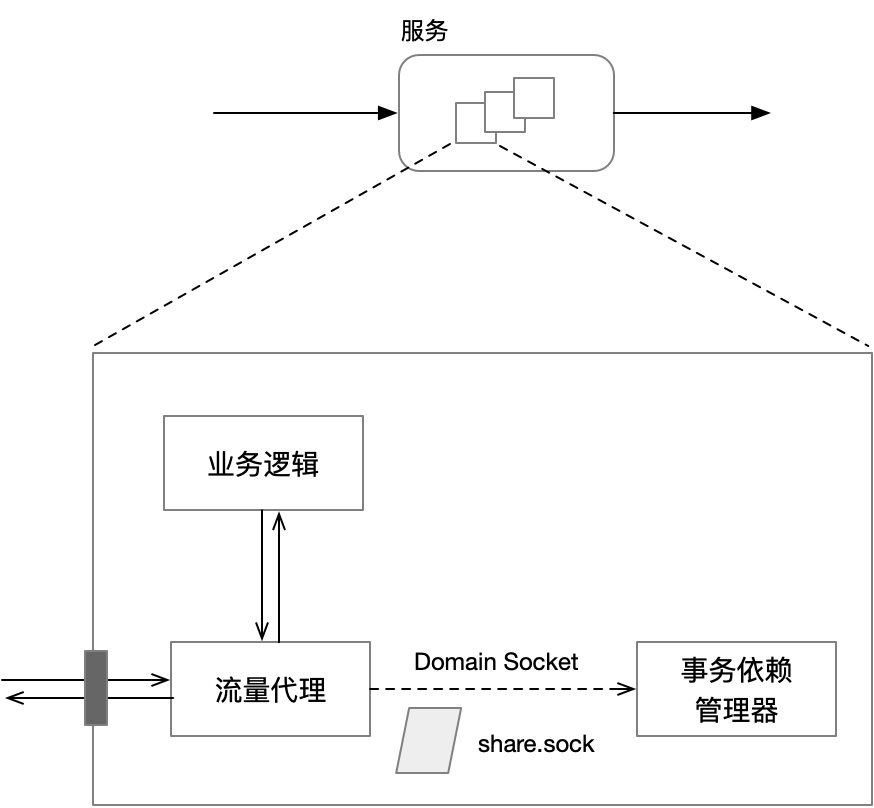
\includegraphics[width= 0.7\textwidth]{image/instance_model.png}
  \caption{微服务实例模型}
  \label{fig:instance_model}
\end{figure}

\subsection{服务生命周期管理器}
想要对运行于Istio框架之上的服务进行动态更新,需要对原先服务的生命周期模型进行了扩展,定义了对应的服务生命周期管理器,提供监听服务状态、管理服务生命周期的基本功能。

当前Istio框架的运行环境与容器编排系统Kubernetess\footnote{Kubernetes home page: https://kubernetes.io/}相耦合,服务以容器的形式运行在其之上。因此,服务生命周期管理器的实现主要利用Kubernetes中提供的自定义资源CRD(Custom Resource Definition)功能,其实现原理称为控制器模式,如图\ref{fig:reconcile_loop}所示。用户通过声明式命令对期望状态进行描述,控制器对比期望状态与系统实际的运行状态,如果有出入则通过自定义的调谐逻辑(Reconcile)驱使实际状态调整为期望状态。

\begin{figure}[!htbp]
  \centering
  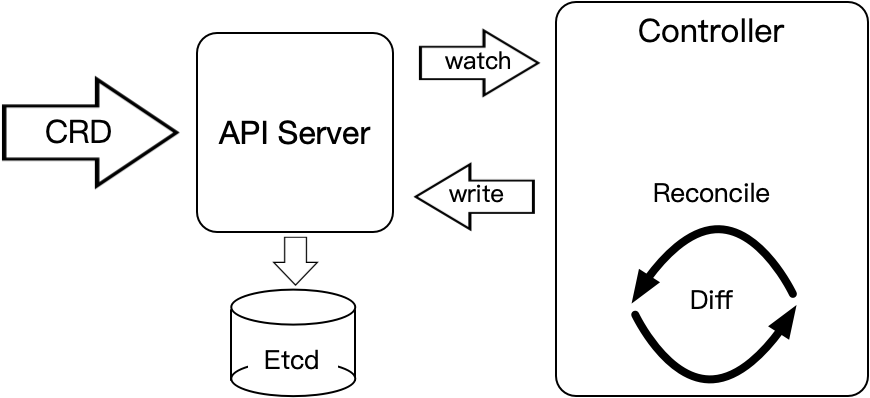
\includegraphics[width= 0.8\textwidth]{image/reconcile_loop.png}
  \caption{控制器模式}
  \label{fig:reconcile_loop}
\end{figure}

通过对系统中服务的概念进行抽象,定义出与服务生命周期相匹配的自定义资源,称之为托管服务MS(Managed Service)。托管服务是一个抽象资源,每个托管服务包含了服务名称、服务的路由版本和当前状态等信息,负责对系统中的某一服务进行管理,对应服务在系统中可能存在多个版本的运行实例。当用户主动发起对托管服务的状态变更请求,如切换新版本、撤销旧版本等请求时,托管服务的控制器将监听到相应的变化,然后通过更新系统中的相关资源配置,驱使服务向目标状态进行跳转;若出现异常,调谐逻辑将重新执行,直至服务的状态跳转成功。

托管服务资源的定义很好地与服务生命周期的概念完成了匹配,对外屏蔽了内部服务的细节信息,抽象出对应的服务运行状态,对内又可以很好地对各个服务实例的生命周期进行管理。

由前一章节对服务生命周期模型的讨论可知,用户对目标更新服务的动态更新操作与服务当前所处的状态存在着密不可分的关系。因此,我们将动态更新的相关算法整合到托管服务的调谐逻辑之中,在完成动态更新中关键的版本更新和撤销操作的同时,驱使服务状态进行相应的跳转。下面将具体对实现的版本更新和版本撤销算法进行介绍,为方便说明,这里仍以\ref{sec:example}节中引入的系统为例。

\subsubsection{版本更新}
为了保证动态更新过程中的安全性,即满足定义\ref{def:safety}中的要求,更新算法首先需要对运行中的事务所涉及的服务版本进行标识。因此,我们在头信息中引入自定义字段x-version来进行具体的标识。当调用方向服务发起请求并返回时,利用流量代理模块的拦截功能,在其头信息中添加上带有x-version的服务版本信息,作为事务上下文信息进行返回。随后调用方在接收处理结果时,从头信息提取出事务上下文信息并进行更新本地信息,后续发起远程调用时将利用更新后的信息进行传递,从而完成了对运行时事务的版本标识工作。

如图\ref{fig:convertor_normal_v1}所示,表示Convertor服务在初始版本为v1时,系统的正常运行状态。对于所有向Convertor服务发起调用的请求,在其返回头信息中添加x-version: convertor-v1字段,表征该事务针对于目标更新服务Convertor被标识为v1版本。这里将Convertor服务作为目标更新服务,因此仅关注与Convertor服务相关的字段信息,其它非目标更新服务可类推。

\begin{figure}[!htbp]
  \centering
  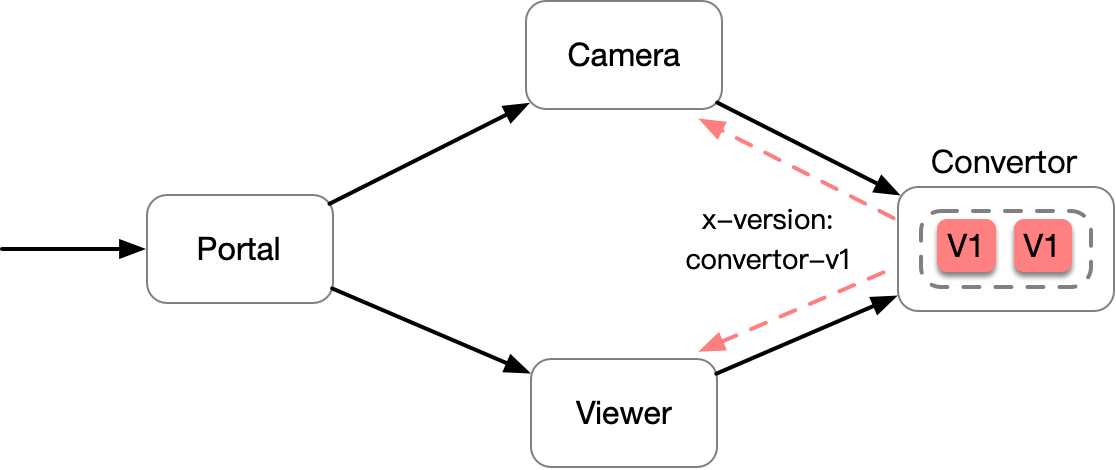
\includegraphics[width= 0.8\textwidth]{image/convertor_normal_v1.png}
  \caption{初始状态下的系统}
  \label{fig:convertor_normal_v1}
\end{figure}

基于运行时事务版本的正确标识,我们可进一步实现服务版本的正确更新。服务被选定为目标更新服务之后,用户需要对新版本进行上线部署工作,服务进入Deployed状态,假定对应的新旧版本标识分别为v2、v1。此时,对流量代理模块中的路由规则进行修改,添加头信息匹配规则:若本次请求头信息中的x-version字段包含特定的版本信息,则将该请求转发往特定版本;否则,默认转发往旧版本,同时在返回头信息中添加对应字段。对应系统的运行状态如图\ref{fig:convertor_prepared_v1v2}所示,虽然系统中的v2版本服务实例已经就绪,但请求全部由v1版本的服务实例进行处理。

\begin{figure}[!htbp]
  \centering
  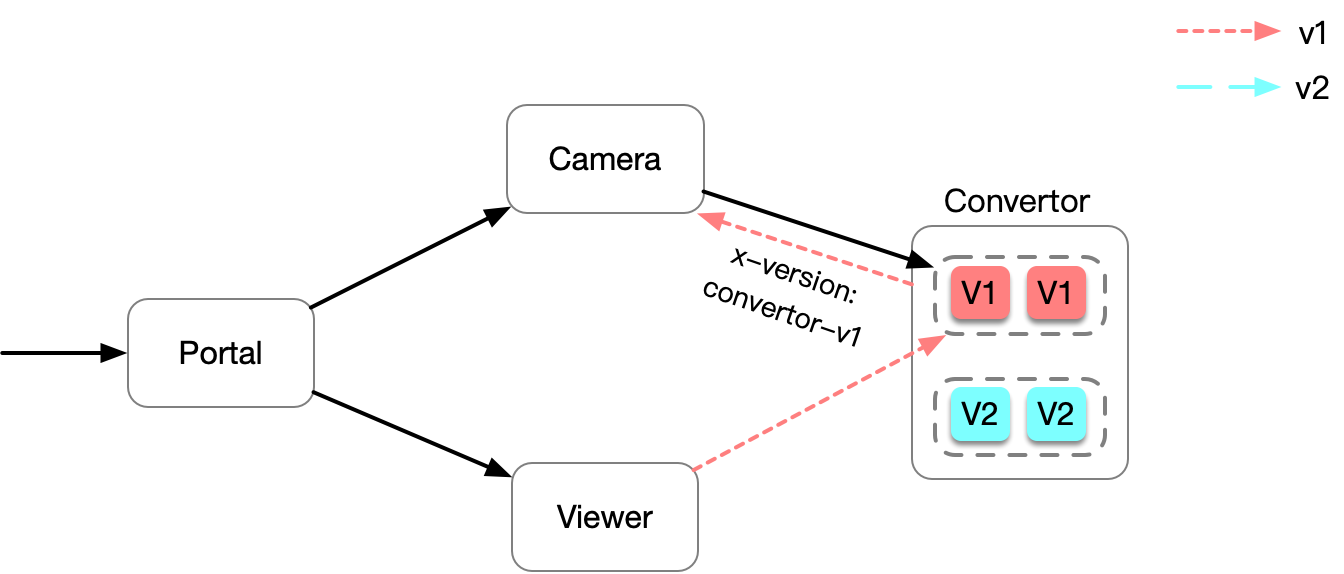
\includegraphics[width= 0.9\textwidth]{image/convertor_prepared_v1v2.png}
  \caption{更新准备前的系统}
  \label{fig:convertor_prepared_v1v2}
\end{figure}

前述的更新准备工作完成后,将原先路由规则中默认转发往旧版本修改为默认转发往新版本。对应系统的运行状态如图\ref{fig:convertor_shift_v1v2}所示,考虑对于任意一个分布式事务T,在规则生效之后,向Convertor服务发起请求,将包括如下几种情况:

\ding{172}若分布式事务T在运行的过程中还未在Convertor服务上发起过子事务,则其请求头信息中将不包含相关的x-version字段。依据生效后的路由规则,此分布式事务T对于Convertor服务的请求,将被转发往新版本;

\ding{173}若分布式事务T在运行的过程中曾经在Convertor服务上发起过子事务,则由前述规则可知,其请求头信息中必然包含了相关的x-version字段。依据生效后的路由规则,此分布式事务T对于Convertor服务的请求,将被转发往与x-version字段具有相同标识的版本实例中;

综上,保证了任一分布式事务T在运行过程中,不会在目标更新服务Convertor的不同版本实例上发起子事务,即满足了动态更新算法对于安全性的要求,同时也使得新生成的分布式事务可以较快地使用到新版本的服务。

\begin{figure}[!htbp]
  \centering
  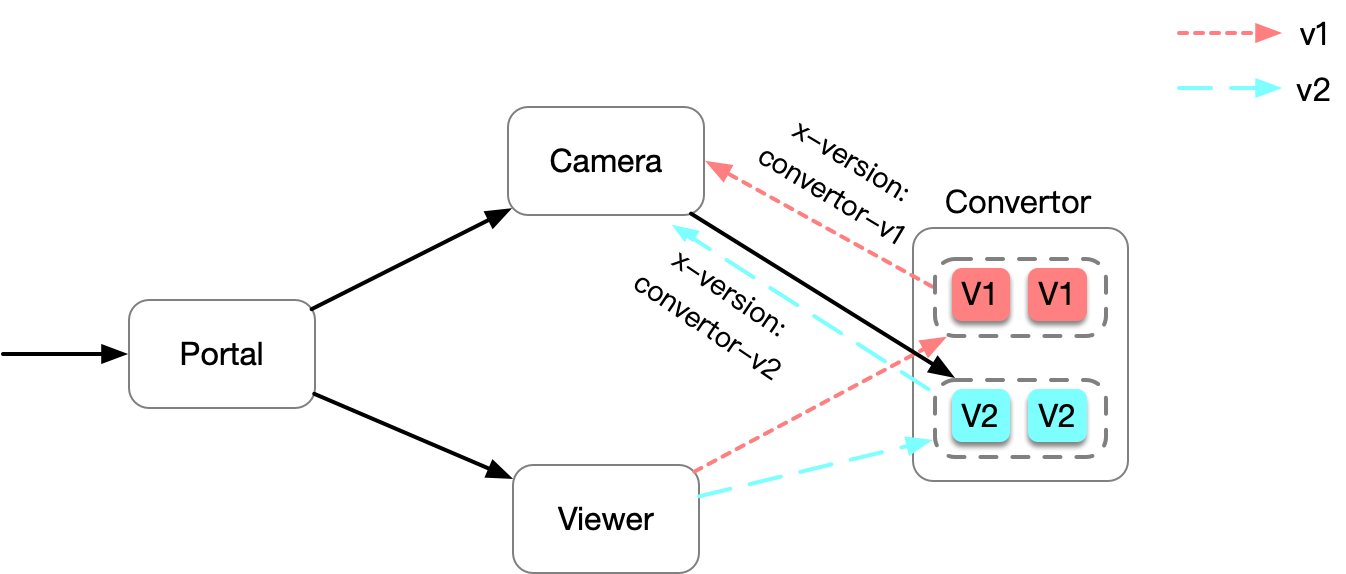
\includegraphics[width= 0.9\textwidth]{image/convertor_shift_v1v2.png}
  \caption{版本更新中的系统}
  \label{fig:convertor_shift_v1v2}
\end{figure}

\subsubsection{版本撤销}
前述的版本更新算法在保证动态更新安全性的基础上,很好地完成了目标更新服务新旧版本请求的正确导向。在此基础上,当收到用户的旧版本撤销请求时,要求版本撤销算法在保证用户请求不会出错的情况下,尽快完成旧版本实例的撤销,及时释放其占用的系统资源。

在正常状态下,当服务收到请求生成事务时,事务依赖管理器将负责对PAST\_SET集合进行更新,保存所有曾经在此服务上发起过子事务的分布式事务的标识,如图\ref{fig:normal_past_set}所示。

\begin{figure}[!htbp]
  \centering
  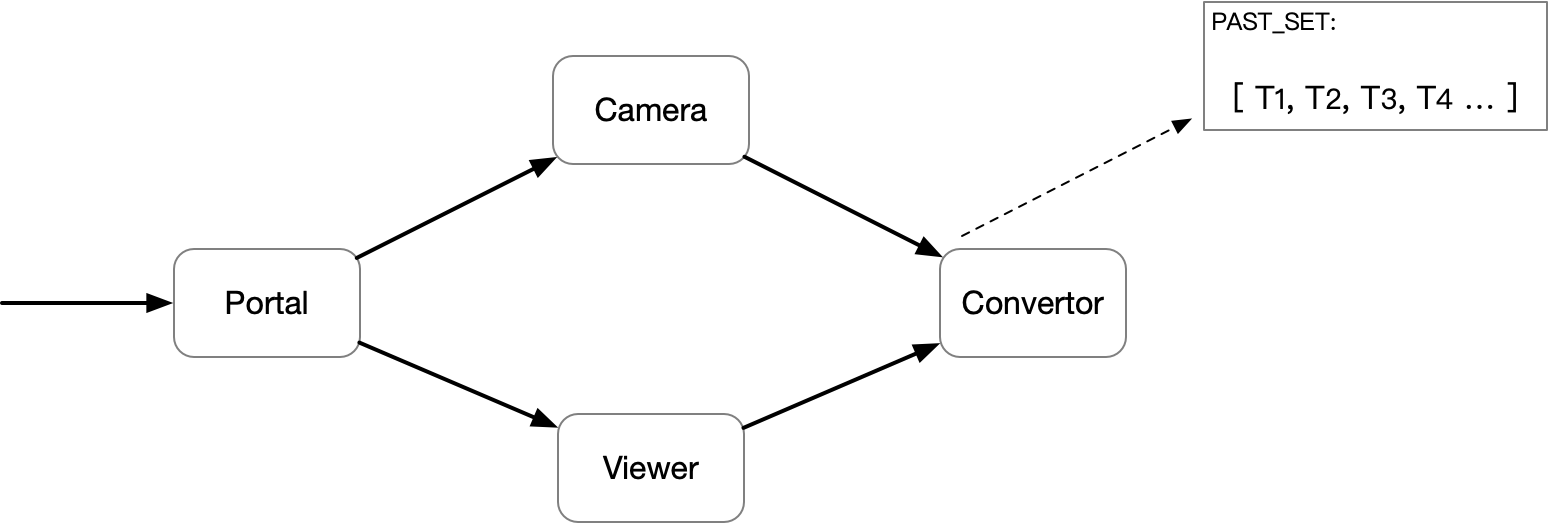
\includegraphics[width= 1.0\textwidth]{image/normal_past_set.png}
  \caption{维护PAST\_SET集合}
  \label{fig:normal_past_set}
\end{figure}

版本撤销算法的关键在于判断:\\


\begin{spacing}{1.0}
\end{spacing}

$\bullet$$\indent$旧版本服务实例不会再为未结束的事务提供服务

\begin{spacing}{2.0}
\end{spacing}

$\bullet$$\indent$旧版本服务实例当前未执行任何事务 \\

\begin{spacing}{1.0}
\end{spacing}

应用文献\cite{ma2011version}中所提出的Freeness更新判断条件\ref{def:Freeness},利用前述的事务依赖管理器维护的PAST\_SET和FUTURE\_SET集合,实现了对应的版本撤销算法,具体包括如下步骤:\\


\begin{spacing}{1.0}
\end{spacing}

$1$$\indent$\textbf{阻塞访问}:当收到旧版本撤销请求时,系统首先阻塞所有向旧版本服务

$\indent$$\enspace$实例发起调用的新生成的分布式事务,即其头信息中不存在标识版本信

$\indent$$\enspace$息的x-version字段。而对于曾经在旧版本服务实例上发起过的子事务的

$\indent$$\enspace$分布式事务,则允许通过。被阻塞的请求将在调用方执行重试,依据前

$\indent$$\enspace$述版本更新算法中路由规则的定义,本次请求将会被转发往新版本的服

$\indent$$\enspace$务实例中,保证了用户请求依然能够被正常地处理,而且不会再有新的

$\indent$$\enspace$分布式事务标识添加到相关的事务依赖管理器所维护的PAST\_SET集合

$\indent$$\enspace$中,对应的系统状态如图\ref{fig:revoke_1}所示;

\begin{spacing}{2.0}
\end{spacing}


\begin{figure}[!htbp]
  \centering
  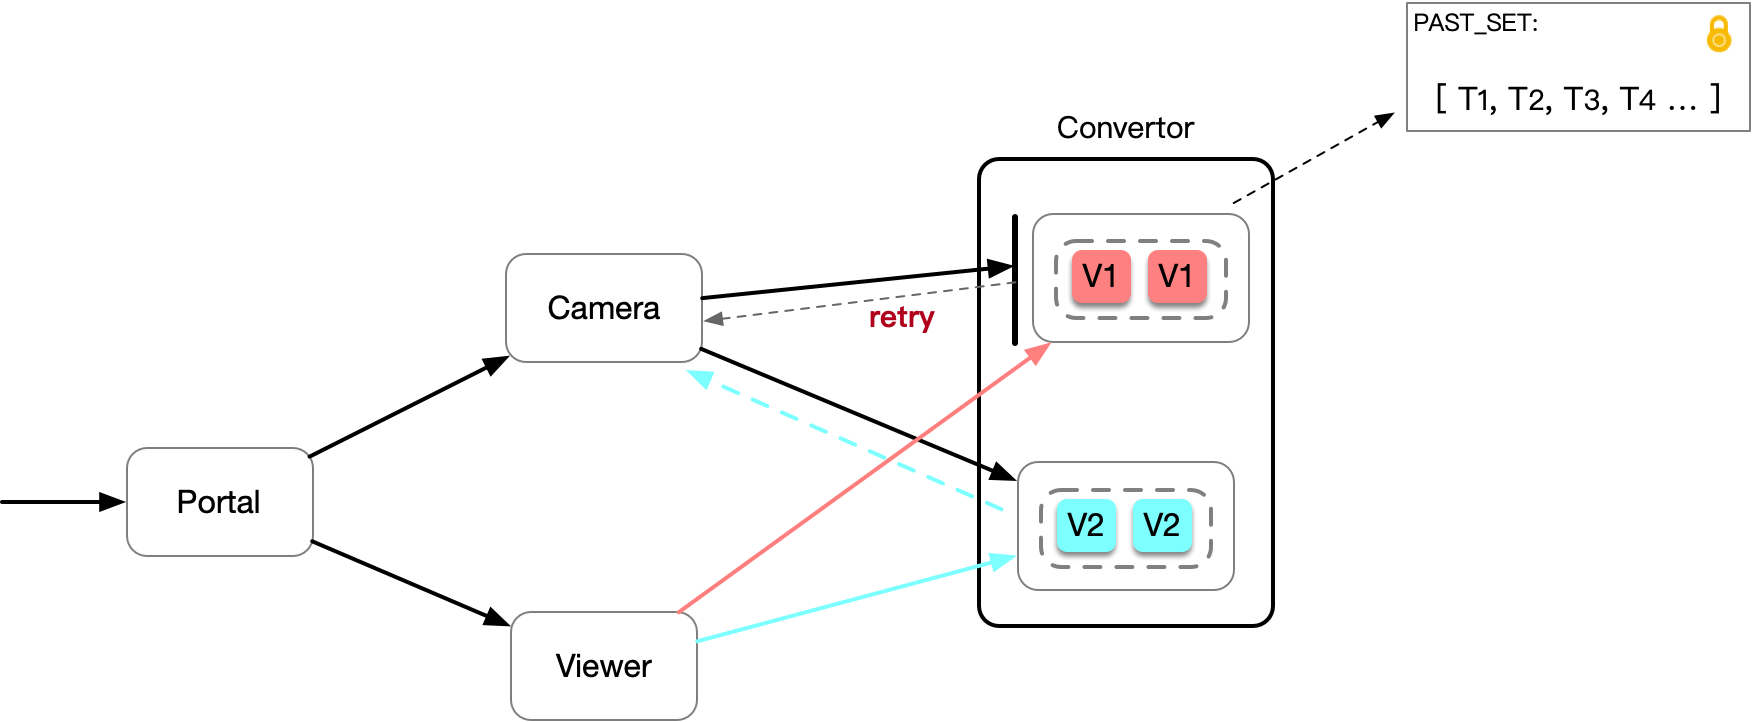
\includegraphics[width= 1.0\textwidth]{image/revoke_1.png}
  \caption{阻塞访问}
  \label{fig:revoke_1}
\end{figure}

\begin{spacing}{2.0}
\end{spacing}

$2$$\indent$\textbf{同步状态}:由前述可知,分布式事务将来是否会调用目标更新服务的状

$\indent$$\enspace$态信息,保存于系统内的各个服务实例中。目标更新服务可利用本地维

$\indent$$\enspace$护的PAST\_SET集合,向依赖于自身的相关服务发起请求,同步相关服

$\indent$$\enspace$务的事务状态信息,便可得到相应的FUTURE\_SET集合。此集合代表所

$\indent$$\enspace$有将来会向目标更新服务发起请求的分布式事务标识集合,同步过程如

$\indent$$\enspace$图\ref{fig:revoke_2}所示,其中的红色虚线段表示具体请求过程:

\begin{spacing}{2.0}
\end{spacing}

\begin{figure}[!htbp]
  \centering
  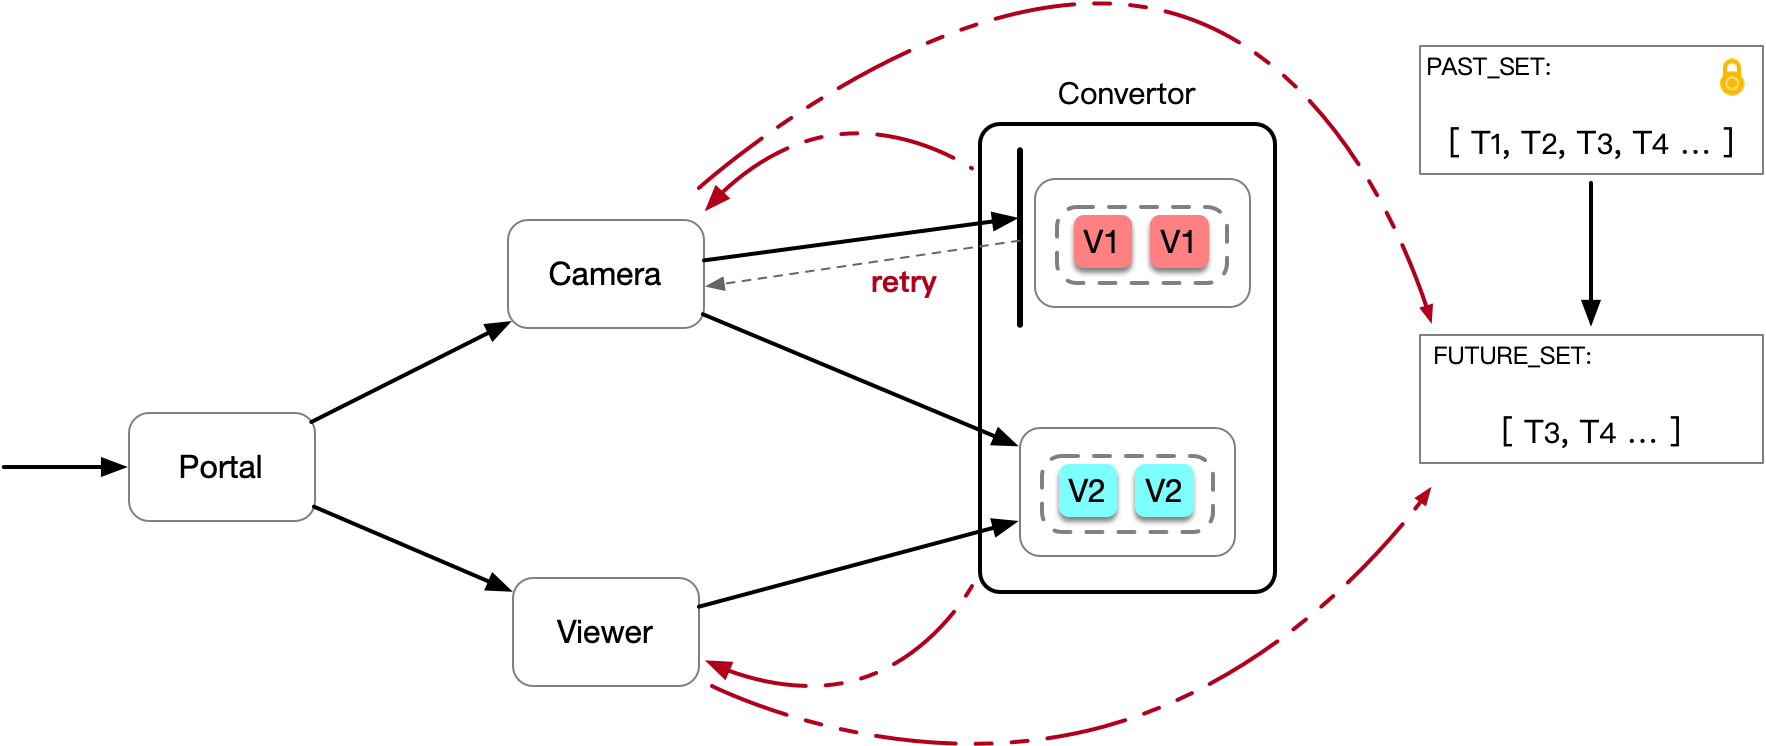
\includegraphics[width= 1.0\textwidth]{image/revoke_2.png}
  \caption{同步状态}
  \label{fig:revoke_2}
\end{figure}

\begin{spacing}{2.0}
\end{spacing}

$3$$\indent$\textbf{等待撤销}:基于前一步骤所得到的FUTURE\_SET集合,并结合实例本地

$\indent$$\enspace$事务依赖管理器所维护的相关信息,撤销算法如图\ref{fig:revoke_3}所示,可执行进

$\indent$$\enspace$一步的判断:若接收到的FUTURE\_SET集合为空,表示针对当前所有调

$\indent$$\enspace$用过旧版本服务实例的分布式事务,均不会再向目标更新服务发起请求

$\indent$$\enspace$,因此只需等待当前旧版本实例上的事务执行结束,即可执行撤销操作

$\indent$$\enspace$,算法执行结束;否则,即表示当前系统中的分布式事务在将来仍会使

$\indent$$\enspace$用到旧版本的服务实例,此时撤销算法流程将进入等待状态,待所有

$\indent$$\enspace$FUTURE\_SET集合中的分布式事务均完成调用后,对PAST\_SET集合进

$\indent$$\enspace$行更新,并重新执行前一步骤,以重新同步相关的分布式事务状态。 \\

\begin{spacing}{2.0}
\end{spacing}

\begin{figure}[!htbp]
  \centering
  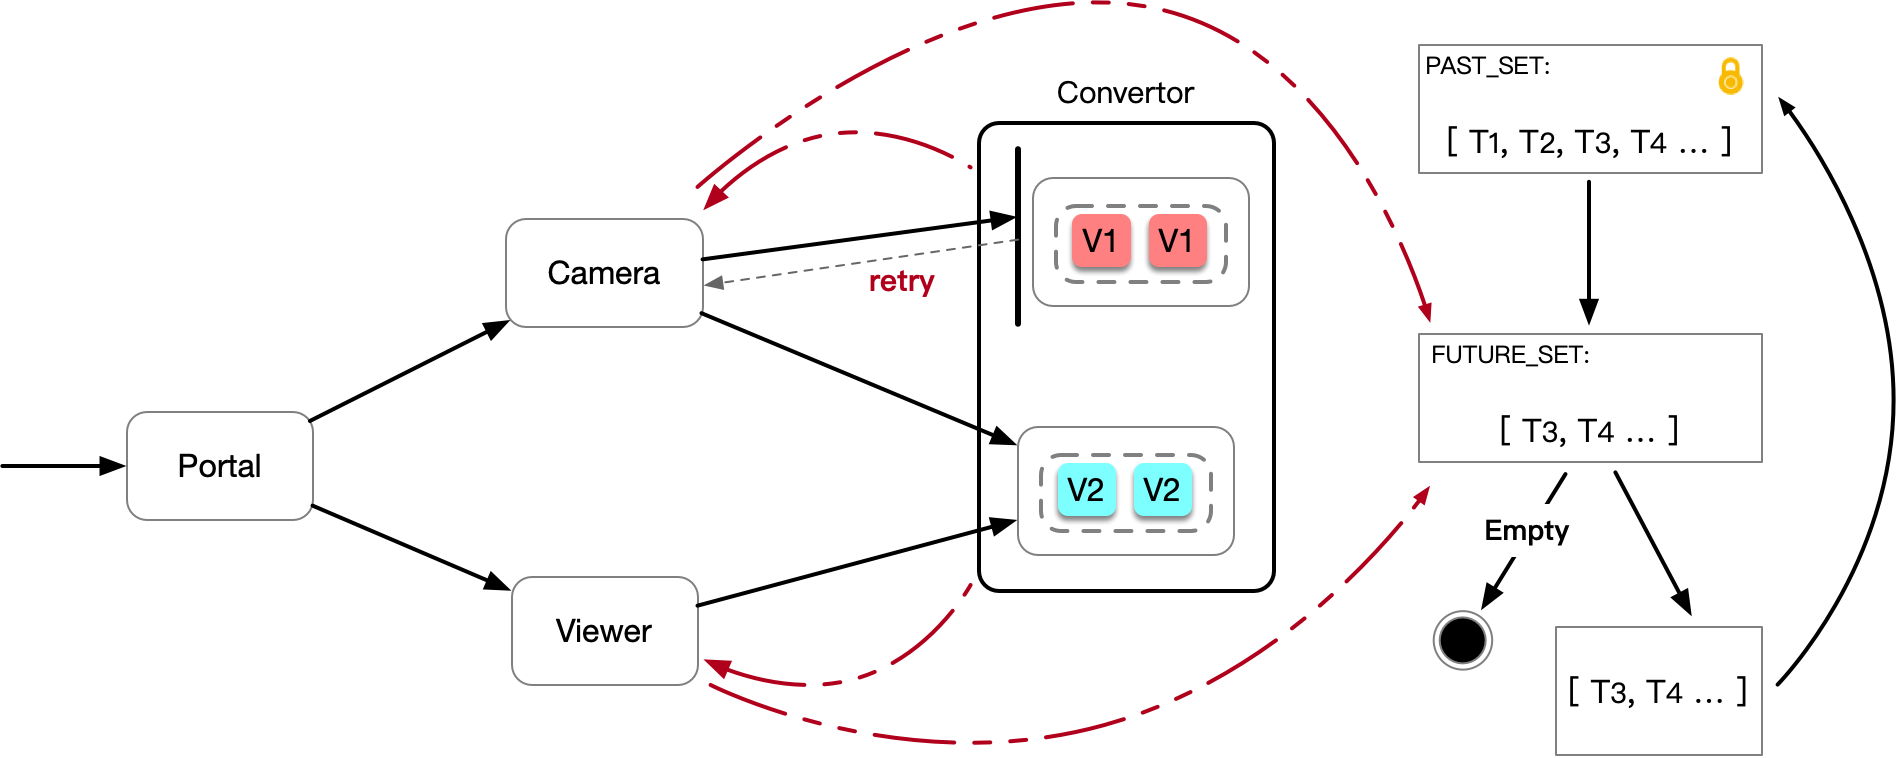
\includegraphics[width= 1.0\textwidth]{image/revoke_3.png}
  \caption{等待撤销}
  \label{fig:revoke_3}
\end{figure}

\begin{spacing}{1.0}
\end{spacing}

版本撤销算法利用本地维护的相关事务依赖信息,通过相关的同步请求来收集到具体的分布式事务状态信息,正确判断服务能否被撤销,保证撤销操作的及时性,而且不会阻塞正常的业务请求,对系统的干扰性较小。

\subsection{更新控制模块}
前述的相关模块为系统提供了支持动态更新的核心能力,为使系统具有更好的操作性,定义了更新控制模块。

更新控制模块作为系统与用户的交互工具,屏蔽系统内部服务的详细运行信息的同时,对外暴露相关的管理接口。用户可通过接口来进行服务状态的查询,以及发起相关的动态更新请求,系统可自动完成动态更新过程,无需额外的人工操作。

\section{系统模块交互}
上一节具体对扩展模块的内部结构及每个模块的功能进行了介绍,本节将重点描述系统运行时各个模块之间的交互关系。

图\ref{fig:update_sequence}展示了版本更新过程的时序图。用户在完成更新前的相关准备工作之后,向更新控制模块发起更新请求。更新控制模块向运行平台的$API~Server$发送相关资源的修改请求,而服务生命周期管理器将监听到相应的资源变化,进入相应的调谐逻辑。调谐逻辑中通过对路由规则进行更新,利用Istio框架前述的配置分发功能,对所有相关服务实例的流量代理模块进行行为配置,以驱使服务的状态完成跳转。

图\ref{fig:revoke_sequence}则展示了版本撤销过程的时序图。同样由用户向更新控制模块发起撤销请求,再由服务生命周期管理器进行相应的处理。此时服务生命周期管理器将进一步与目标更新服务的事务依赖管理模块进行交互,执行前述的版本撤销算法,使得服务达到目标Freeness条件。

\begin{figure}[!htbp]
  \centering
  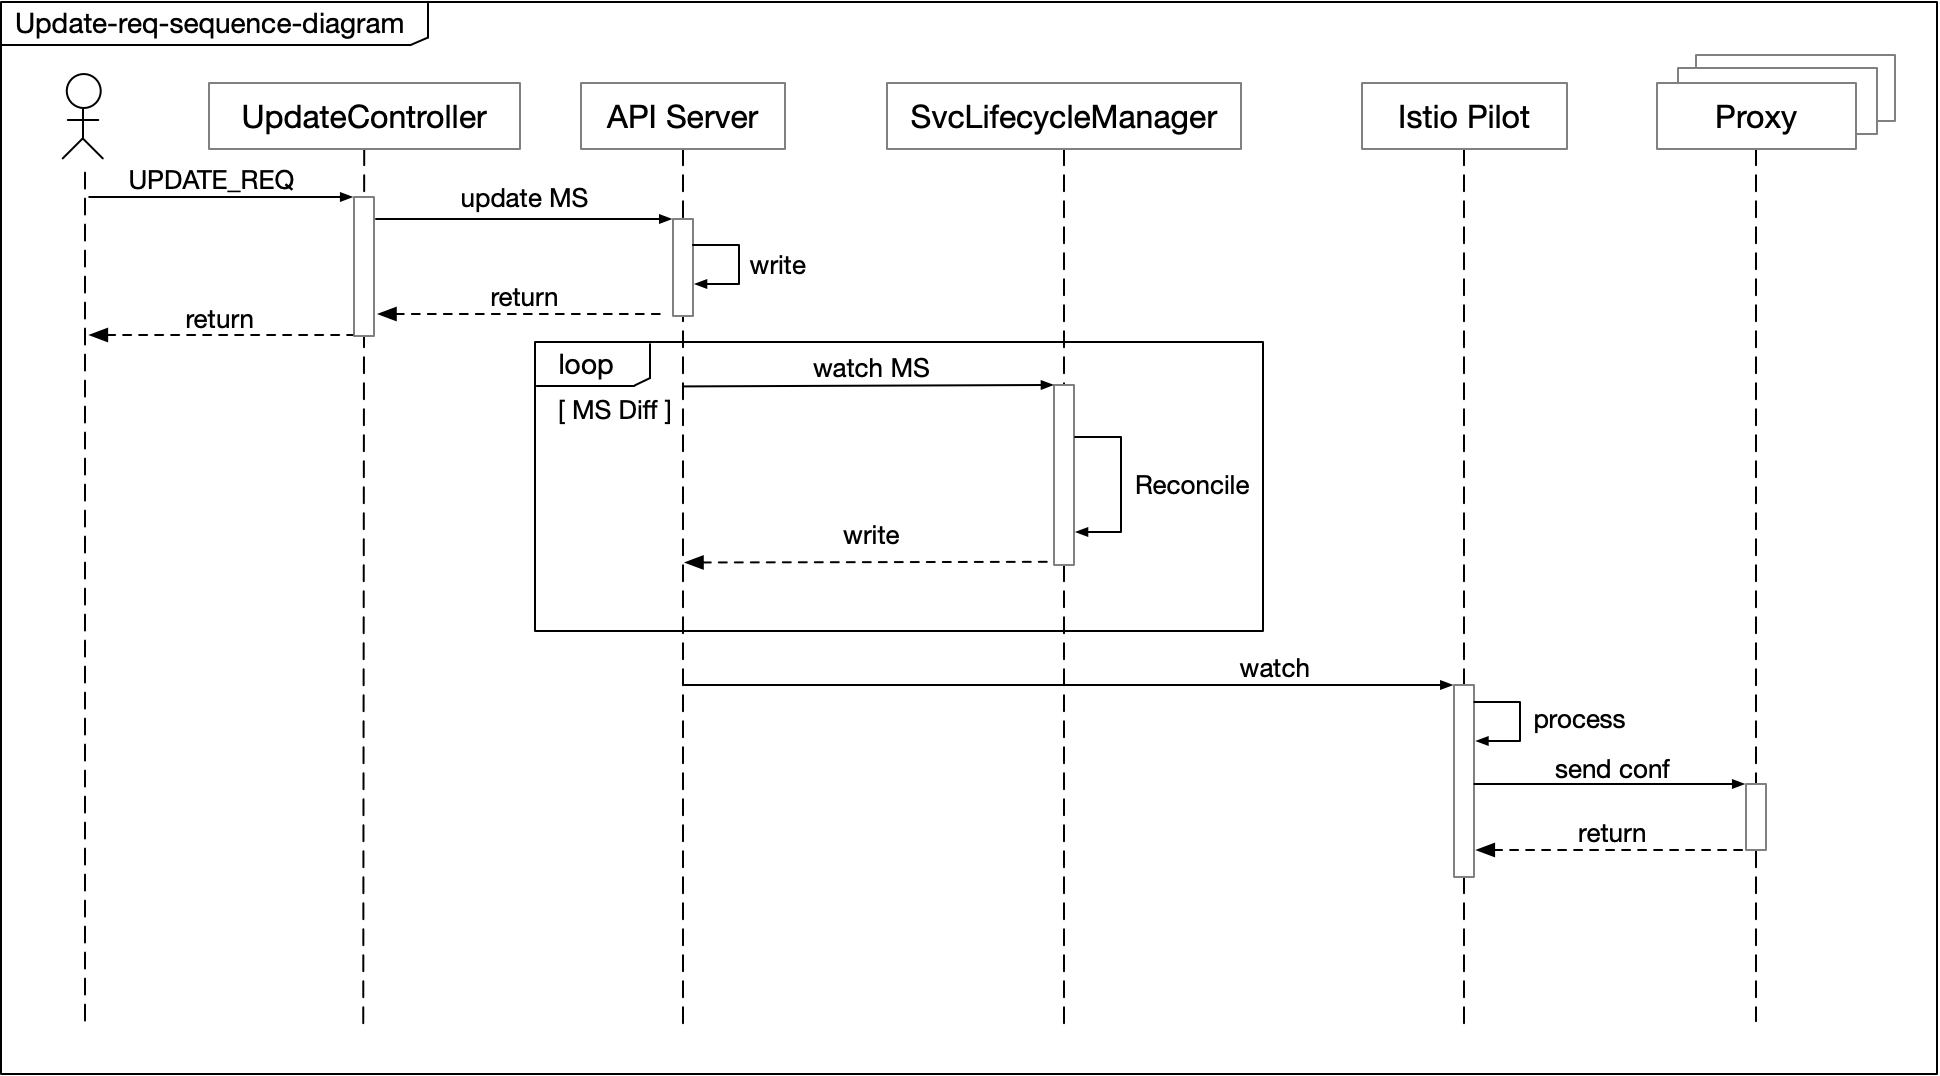
\includegraphics[width= 1.0\textwidth]{image/update_sequence.png}
  \caption{版本更新时序图}
  \label{fig:update_sequence}
\end{figure}

\begin{figure}[!htbp]
  \centering
  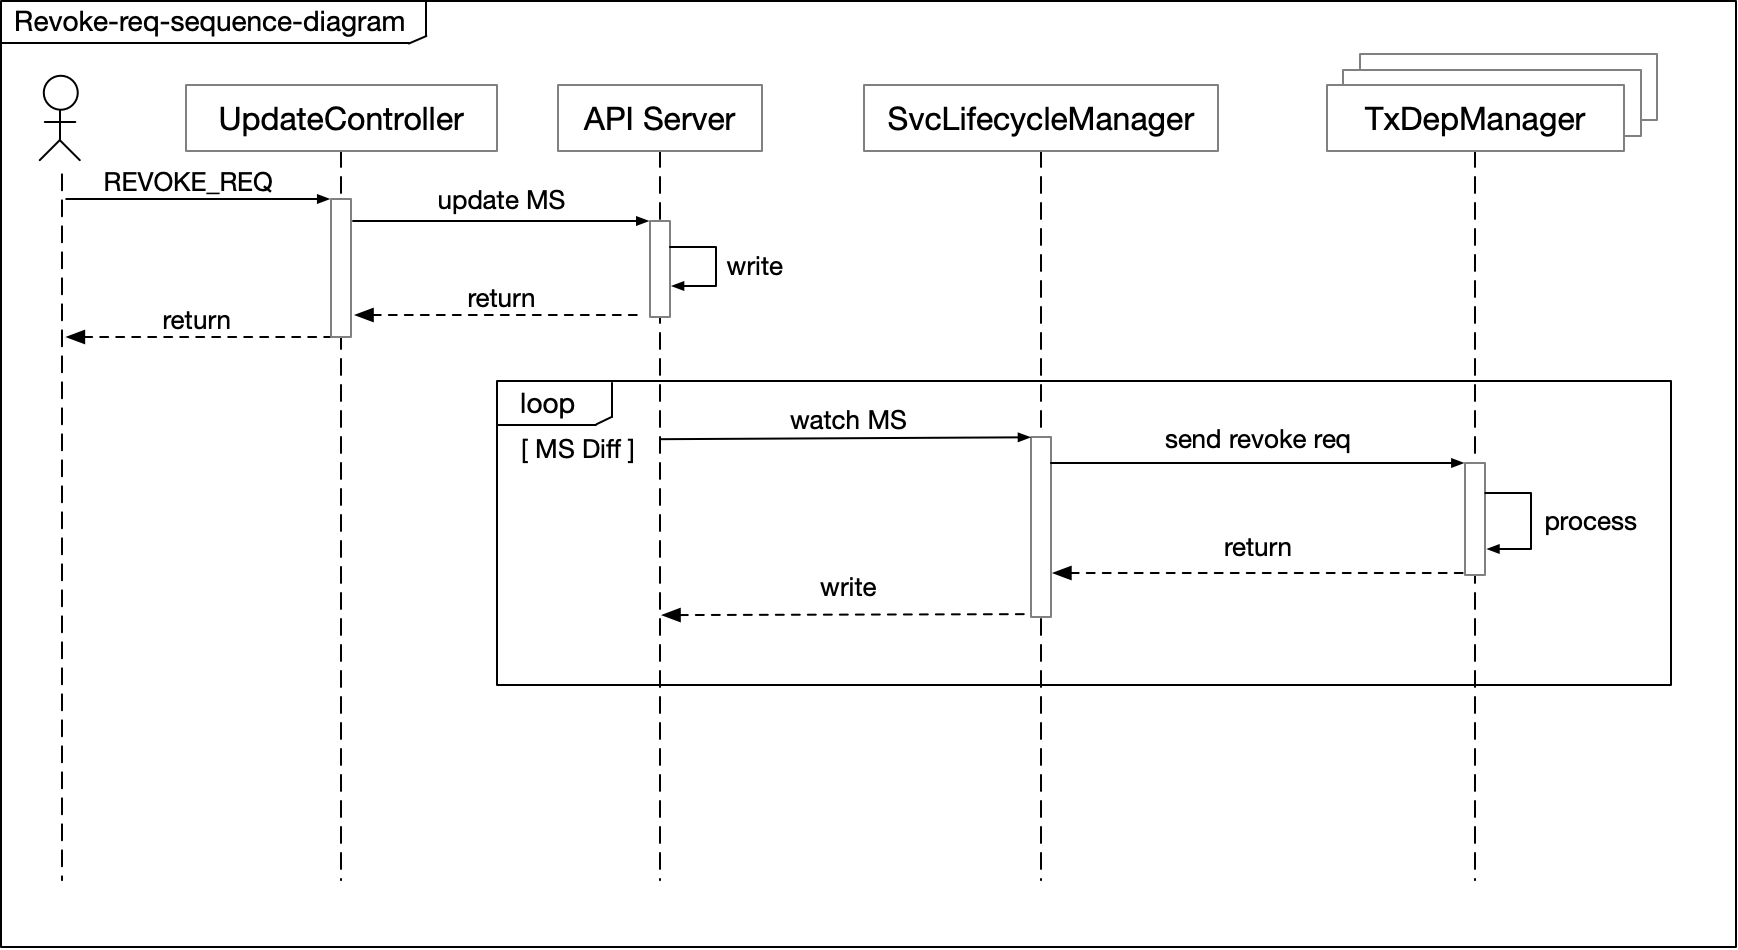
\includegraphics[width= 1.0\textwidth]{image/revoke_sequence.png}
  \caption{版本撤销时序图}
  \label{fig:revoke_sequence}
\end{figure}

\section{本章小结}
本章基于前一章节所提出的VCIM方法,实现支持动态更新的微服务系统。首先,我们对系统的设计实现进行了概述,对系统的设计目标和准则进行了说明。然后本章对三个扩展模块的实现及其模块内部结构进行了详细的介绍,其中包括事务依赖管理器如何对事务进行拦截和管理,为系统支持动态更新提供基础信息;服务生命周期管理器如何对服务的状态进行扩展,版本更新和版本撤销算法如何完成整合,保证动态更新过程的一致性;更新控制模块如何完成用户与系统间的解耦,为用户提供相关的更新管理功能。最后,重点介绍了系统运行时各个模块间的交互关系。

%%%%%%%%%%%%%%%%%%%%%%%%%%%%%%%%%%%%%%%%%%%%%%%%%%%%%%%%%%%%%%%%%%%%%%%%%%%%%%%
\chapter{案例研究与实验评估}\label{chapter_experiments}
为了验证前述的微服务动态更新系统实现方案是否满足动态更新过程的相关准则,本章将利用一个实际场景下的分布式微服务系统进行实验。实验将针对不同的动态更新算法,同时在特定算法实验中对多个服务进行动态更新,在安全性、及时性和干扰性三个方面的性能进行评估和比较。

\section{案例介绍}
这里使用的分布式微服务系统,是一个面向开发日的台风演示系统。该系统模拟2018年的第18号台风Rumbia,将台风从生成发展到最后结束的运行轨迹进行展示,同时系统通过对雨情和风情的相关服务进行查询,整合了台风及其途径城市的详细信息,为用户提供展示功能。具体来说,用户可通过该演示系统,直观地看到当前台风的运行轨迹。当台风的影响范围波及某个具体的城市时,系统将对所在城市的相关雨情和风情服务进行查询,并进行展示预警。该系统的静态依赖关系如图\ref{fig:typhoon_example}所示:

\begin{figure}[!htbp]
  \centering
  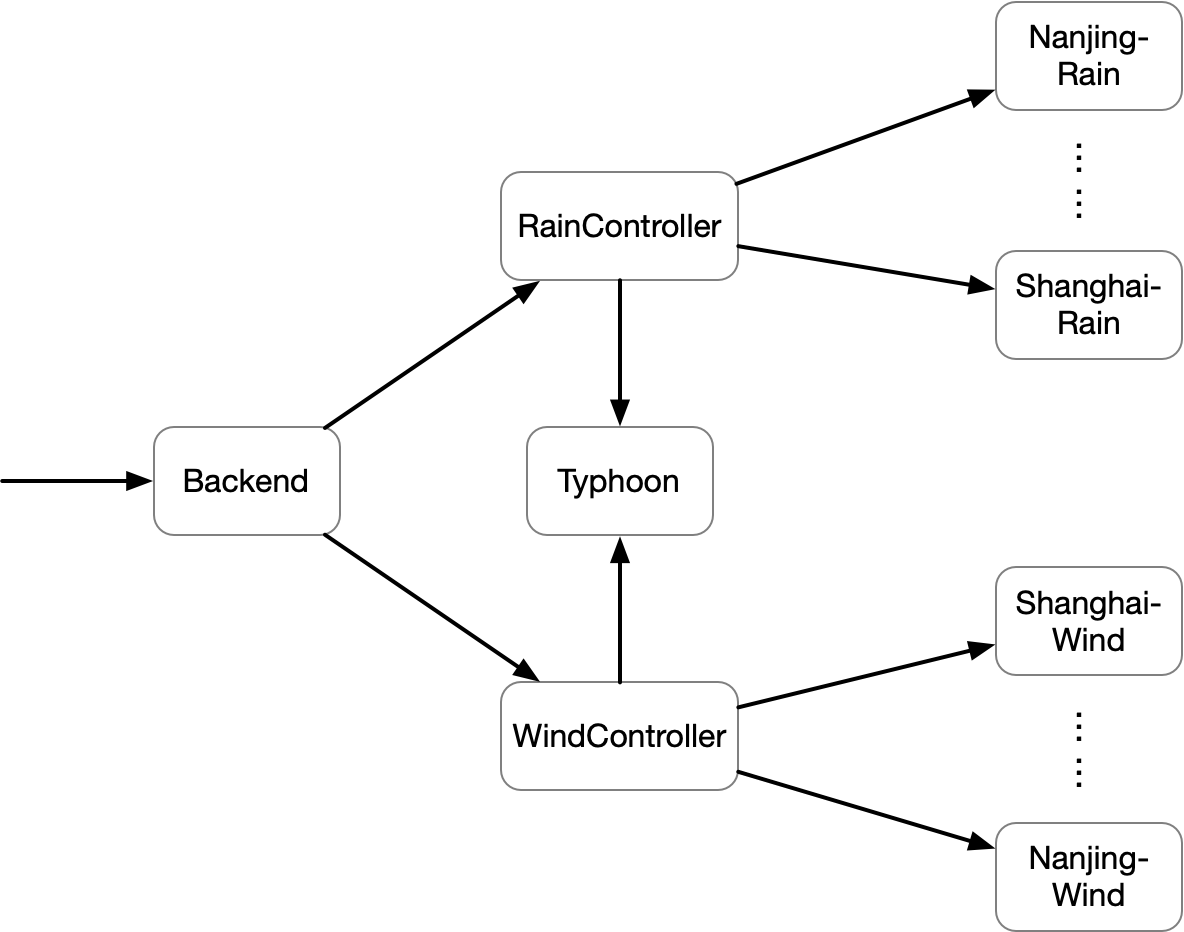
\includegraphics[width= 1.0\textwidth]{image/typhoon_example.png}
  \caption{台风系统静态依赖关系图}
  \label{fig:typhoon_example}
\end{figure}

台风演示系统中,部分主要服务提供的功能如下:\\

\begin{spacing}{1.0}
\end{spacing}

$\bullet$$\indent$\textbf{Backend}$\indent$服务负责整合包括台风强度、位置等详细信息,以及途径影响城

$\indent$$\enspace$市的具体信息。

\begin{spacing}{2.0}
\end{spacing}

$\bullet$$\indent$\textbf{RainController}$\indent$服务负责整合所有台风波及城市具体的雨情信息。

\begin{spacing}{2.0}
\end{spacing}

$\bullet$$\indent$\textbf{WindController}$\indent$服务负责整合所有台风波及城市具体的风情信息。

\begin{spacing}{2.0}
\end{spacing}

$\bullet$$\indent$\textbf{Typhoon}$\indent$服务负责提供台风当前的详细信息,包括经纬度位置、强度和速

$\indent$$\enspace$度等。

\begin{spacing}{2.0}
\end{spacing}

$\bullet$$\indent$\textbf{xx-Rain(Wind)}$\indent$服务负责具体xx城市的雨情(风情)信息。 \\

\begin{spacing}{1.0}
\end{spacing}

服务间的交互时序图如图\ref{fig:typhoon_sequence}所示(已省略去部分非关键服务):

\begin{figure}[!htbp]
  \centering
  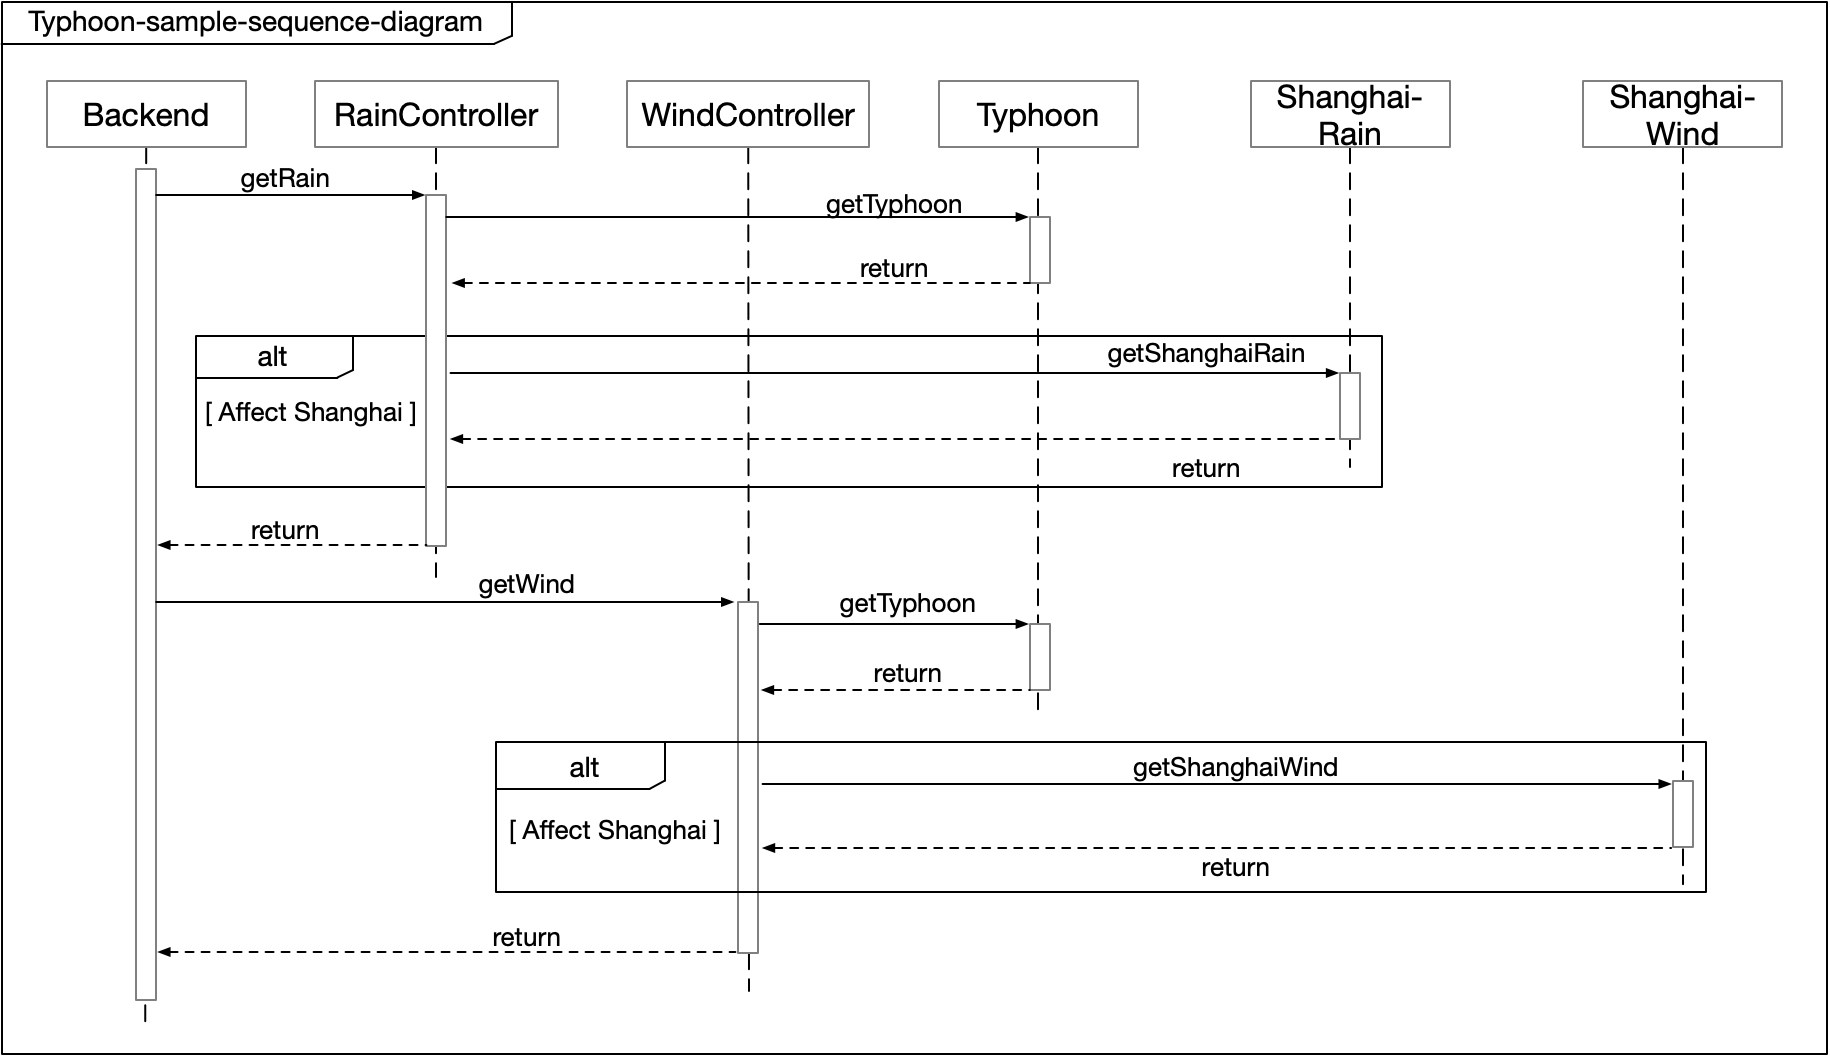
\includegraphics[width= 1.0\textwidth]{image/typhoon_sequence.png}
  \caption{台风系统时序图}
  \label{fig:typhoon_sequence}
\end{figure}

\section{实验环境与设计}

\subsection{实验环境}
我们将使用上述的台风演示系统来对本文实现的动态更新技术进行评估,为了更好地模拟真实场景下的分布式微服务系统,本次实验将台风演示系统中的16个服务部署于Kubernetes系统之上,由其进行容器运行时的编排,具体的环境配置为:

物理节点机器硬件配置:24核 2.5GHz CPU,64GB内存,1T硬盘,千兆以太网卡

软件环境配置:Ubuntu 20.04.1 LTS,Kubernetes v1.17.14

\subsection{实验设计}\label{sec:experiment_design}
在台风演示系统的实际运行中,多个服务均有相应的更新需求:\\

\begin{spacing}{1.0}
\end{spacing}

$1.$$\indent$Typhoon服务可能需要通过更新来更新数据或修复错误。

\begin{spacing}{2.0}
\end{spacing}

$2.$$\indent$RainController、WindController服务可能需要通过更新来整合更多的城市

$\indent$$\enspace$服务信息。

\begin{spacing}{2.0}
\end{spacing}

$3.$$\indent$xx-Rain(Wind)服务可能需要通过更新来引入新的信息提供方式。 \\

\begin{spacing}{1.0}
\end{spacing}

对于上述需求,系统开发人员希望能够在完成代码的改动之后,不停止系统运行的前提下,完成目标服务的动态更新。

服务间的静态依赖关系如\ref{fig:typhoon_example}所示,其中Typhoon服务在实验案例中处于整个调用层次的第三层,可在其之上发起子事务的服务包括RainController和WindController,整个分布式事务的根事务在Backend服务上发起,因此四个服务的调用关系近似形成一个“菱形”的关系。对于Quiescence算法来说,当Typhoon服务需要进行动态更新时,需要保证EPS(Typhoon)集合中的所有服务均属于Passive状态,即Backend、RainController、WindController都必须达到Passive状态,显然这将对系统造成很大的干扰,并且更新所耗费的时间也会很长,对应于动态更新的干扰性和及时性。而对于VCIM算法来说,只需依据Typhoon服务上事务的相关信息以及同步相关服务上事务的运行状态,即可完成动态更新。因此选择Typhoon服务进行动态更新可以有效地评估不同更新算法的及时性和干扰性。另一方面,对于常见的微服务部署方案来说,其考虑新版本服务的快速部署更新,对应的算法为直接切换版本算法(Direct)。若Typhoon服务需要进行动态更新,系统会在新版本服务就绪后,直接进行版本切换更新,显然,若更新的时机发生在RainController发生之后,且在开始调用WindController之前,那么本次更新将导致系统出现不一致的情况,而Quiescence和VCIM则不会出现不一致的情况,对Typhoon服务进行更新对验证各个算法的安全性具有实际意义。因此在进行单个服务更新实验中,将选择Typhoon服务作为目标更新服务。

在具体的应用场景下,系统内不同的微服务可能由独立的团队来开发管理,因此多个服务可能同时存在更新需求。为了验证本文实现方法的有效性以及服务生命周期模型的独立性,将同时对系统中多个服务进行更新,多服务更新实验中选择WindController服务和Typhoon服务作为目标更新服务。

在具体的实验设置方面,将<算法,请求间隔,实验目标>称为一组实验,其中算法包括Quiescence、VCIM、VCIM-MUL和相应的基准算法,其中Quiescence算法与具体更新的服务数量无关,而VCIM和VCIM-MUL则分别表示应用VCIM对单个服务和多个服务进行更新;请求间隔包括1500ms、750ms、500ms、300ms、150ms、100ms,请求间隔表示系统收到请求的时间间隔,用来表征系统的负载状况,请求间隔越小说明系统负载越大;实验目标则包括了安全性、及时性和干扰性三个方面。

针对每一组实验,将分别独立地进行5次。每次实验将依据对应的请求间隔,不断地向系统发起请求,一共发送80次,同时在第20个请求处,向系统中的目标更新服务发起动态更新请求。在单服务更新实验中,仅在第20个请求处,额外向系统发起一次动态更新请求;而在多服务更新实验中,在第20个请求处,针对不同的目标更新服务,额外向系统发起两次动态更新请求。此时可以保证系统中已经存在多个运行时分布式事务,可以更好地模拟真实状态下的分布式微服务系统,确保实验的合理性和公平性。

\section{实验分析}
在实际的应用系统中,当运维人员尝试对其中的服务进行动态更新时,动态更新的前后系统的运行时事务是否安全、更新所需要耗费的时间以及整个更新过程对系统会造成多大的干扰,这些都是其评价动态更新算法的重要标准。因此本章的实验将从安全性(Safety)、及时性(Timeliness)和干扰性(Disruption)三个方面,进行具体的评测。

\subsection{安全性(Safety)}
安全性表示在服务进行动态更新的过程前后,系统处理正在运行时的事务和后续将要发生的事务都应满足一致性,即逻辑正确性。不同的动态更新算法对于安全更新点的定义各不相同,因此对于安全性的满足也并不一致。

安全性实验针对前述的三种动态更新算法,分别按照对应的实验设置来进行。例如实验<Direct,1500ms,安全性>表示使用直接切换版本算法进行安全性的实验,模拟的用户请求间隔为1500ms。实验中记录的结果为动态更新过程中出现不一致的用户请求数量,用来表示该算法是否满足安全性。实验结果如表\ref{table:safety_result}所示。

\begin{table}
  \centering
  \begin{tabular}{c|c|c|c|c|c|cp{20mm}}
    %\toprule
    \hline
    \textbf{请求间隔(ms)} & 1500 & 750 & 500 & 300 & 150 & 100 \\
    \midrule
    \hline
    Direct  & 5 &  8  & 12 & 16 & 33 & 50 \\
    \hline
    Quiescence     & 0  &  0  & 0 & 0 & 0 & 0 \\
    \hline
    VCIM     & 0 & 0 & 0 & 0 & 0 & 0 \\
    \hline
    VCIM-MUL     & 0 & 0 & 0 & 0 & 0 & 0 \\
    % \bottomrule
    \hline
  \end{tabular}
  \caption{安全性实验结果}
  \label{table:safety_result}
\end{table}

从表中数据可以看出,直接切换版本算法并未对更新的安全点进行考虑,不能保证动态更新的安全性,且不一致的数量随系统负载的增加而增加。如在请求间隔为500ms时,系统中共出现12次不一致的用户请求数量。而Quiescence算法和本文中实现的VCIM、VCIM-MUL算法在实验中都没有出现不一致的请求,可以保证动态更新的安全性,实验结果和算法的相关理论分析相吻合。

由于直接切换版本算法无法保证动态更新的安全性,因此在后续及时性和干扰性的实验中,我们将仅对Quiescence和实现的VCIM、VCIM-MUL进行实验。

\subsection{及时性(Timeliness)}
及时性表示服务从收到动态更新请求到真正完成动态更新所需要的时间。及时性用于反映动态更新算法的效率,及时性越高对应的服务到达安全更新点所耗费的时间越短,即可以更快地完成动态更新。

在单服务更新的及时性实验中,对于每一组实验都分别记录下服务收到动态更新请求的时间,记为开始时间$time_0$,以及对应完成动态更新的时间,记为结束时间$time_1$,则该组及时性实验的计算结果为$time_1 - time_0$。而在多服务更新的及时性实验中,开始时间$time_0$为两个服务中较早收到动态更新请求的时间,结束时间$time_1$为两个服务中较晚完成动态更新的时间,该组及时性实验的计算结果同样为$time_1 - time_0$。每组实验将独立重复多次进行,通过对多次实验结果进行求和平均,便可得到该组实验的及时性实验结果。

实验结果如图\ref{fig:timeliness}所示。从图中可以看出,两种算法更新目标服务所需要耗费的时间都随系统负载的增加而增加。对于同一系统负载的情况下,Quiescence算法要求的安全点较为严格,更新所耗费的时间较长。而本文中实现的VCIM和VCIM-MUL所耗费的更新时间则要少一些,优于Quiescence算法。同时比较VCIM和VCIM-MUL,可以看出同时更新多个服务并未对更新的及时性造成较大的影响。

\begin{figure}[!htbp]
  \centering
  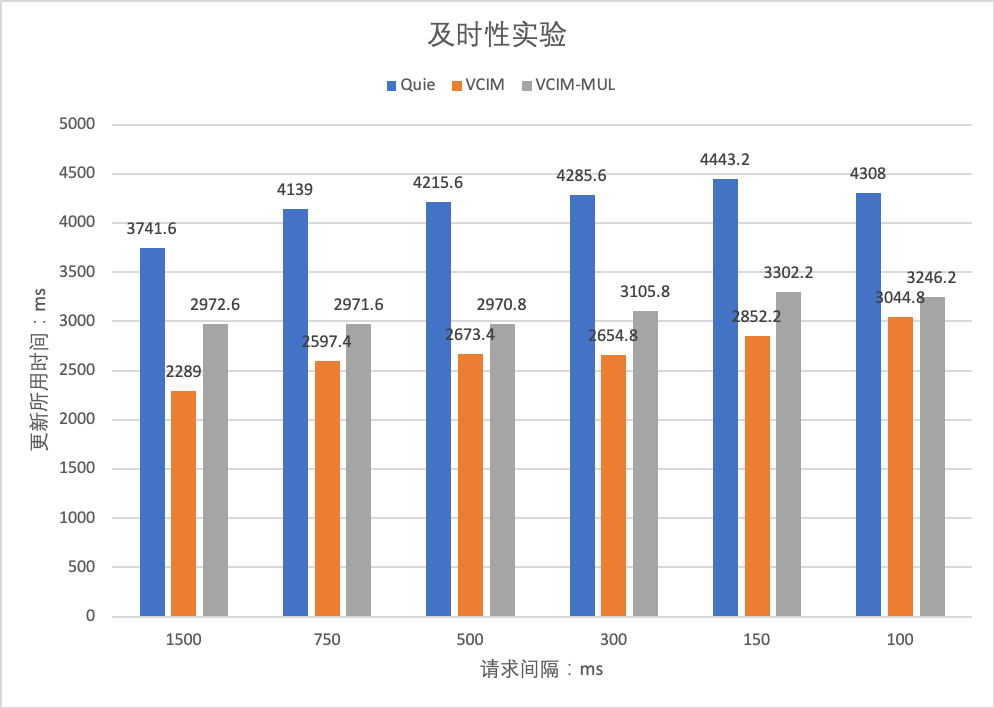
\includegraphics[width= 0.8\textwidth]{image/timeliness.png}
  \caption{及时性实验结果}
  \label{fig:timeliness}
\end{figure}

\subsection{干扰性(Disruption)}
干扰性表示应用动态更新算法给系统正常处理用户请求所导致的中断程度,即相较于没有动态更新请求下,动态更新过程对系统处理用户请求额外增加的时间。某种动态更新算法的干扰性越小,表明该算法更为透明高效。干扰性实验的结果可包括:总干扰性(Total Disruption),平均干扰性(Average Disruption)。

由于需要计算动态更新算法导致额外增加的时间,因此干扰性实验只对受更新影响的分布式事务进行计算。对于某一个分布式事务,其受更新影响当前仅当对应的事务生命周期与服务进行更新的时间段相互重叠。在进行干扰性实验时,首先进行基准组实验,即在没有更新请求的状态下,系统正常处理用户请求的响应时间,重复多次后计算得到平均的响应时间,记为$time_0$。然后对于使用特定更新算法的第j次实验中,统计所有受更新影响的用户请求(分布式事务)的数量,记为$count_j$,以及这些请求对应的响应时间,记为$time_i$。该组实验共进行多次,对应的总干扰性计算结果为:$TotalDisruption = \sum_{j=1}^{5}\sum_{i=1}^{count_j}(time_i - count_j \cdot time_0)$,对应的平均干扰性计算结果为:$AverageDisruption = TotalDisruption / (\sum_{j=1}^{5}count_j)$,其中$count_j$表示在第j次实验中,受更新影响的事务的总数量。

总干扰性和平均干扰性的实验结果分别如图\ref{fig:total_disruption}、图\ref{fig:average_disruption}所示。从干扰性实验结果可以明显看出,由于Quiescence算法在更新过程中需要阻塞外来请求,因此对系统造成的干扰程度较大。而VCIM和VCIM-MUL可以显著降低更新过程对系统的影响,明显优于Quiescence算法。比较VCIM和VCIM-MUL,两者都未对系统造成显著的干扰,表示更新服务的数量对于系统的干扰性较小。

\begin{figure}[!htbp]
  \centering
  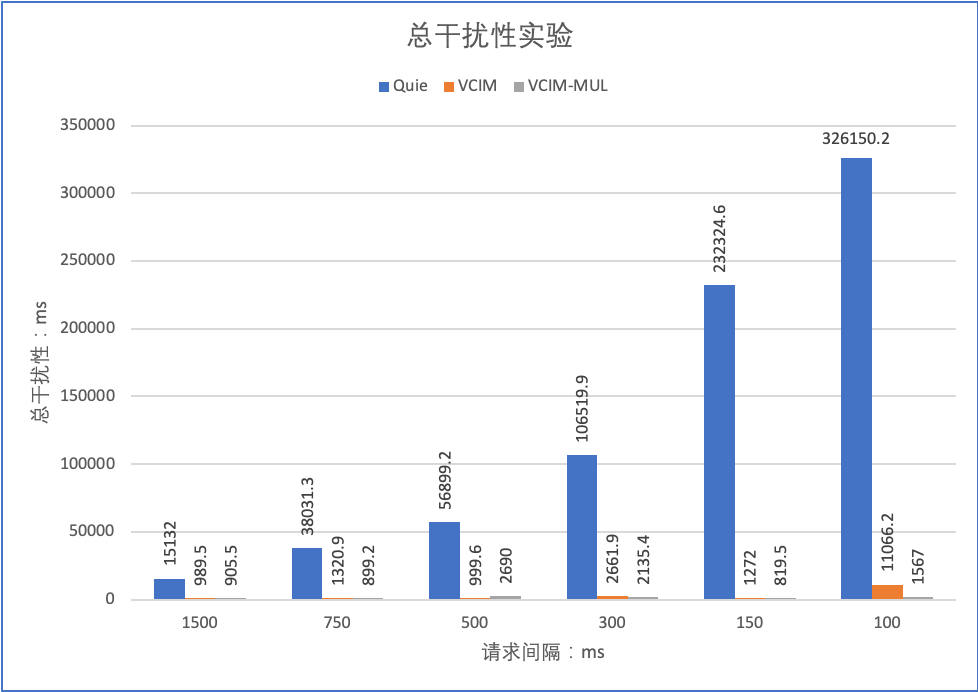
\includegraphics[width= 0.8\textwidth]{image/total_disruption.png}
  \caption{总干扰性实验结果}
  \label{fig:total_disruption}
\end{figure}

\begin{figure}[!htbp]
  \centering
  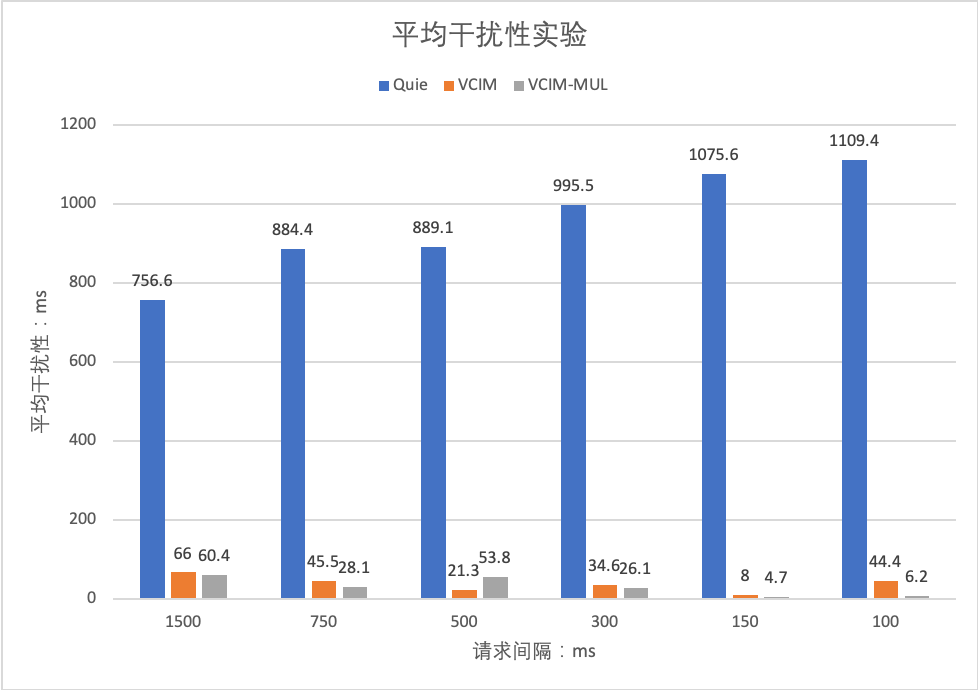
\includegraphics[width= 0.8\textwidth]{image/average_disruption.png}
  \caption{平均干扰性实验结果}
  \label{fig:average_disruption}
\end{figure}

\section{实验结论}
通过上述的实验,我们对各个动态更新算法在安全性、及时性、干扰性三方面进行了性能对比:

\textbf{安全性:}~Quiescence算法和VCIM算法都保证了动态更新过程中的安全性,不会导致系统出现不一致的情况。而直接切换版本算法对应于常见的蓝绿部署和金丝雀部署方案,它们的主要目标是版本的快速更新迭代,并未对安全更新点进行考虑,显然将有可能导致更新过程中系统出现不一致的情况。因此,在安全性方面,Quiescence算法和VCIM算法要优于直接切换版本算法。

\textbf{及时性:}~Quiescence算法利用静态依赖信息,更新需要等待相关事务全部结束,而VCIM算法则利用动态依赖信息,只需保证相关事务不会再次调用到旧版本的目标更新服务即可。因此在及时性方面,VCIM算法要优于Quiescence算法。

\textbf{干扰性:}~由于Quiescence算法更新时对相关服务的状态具有较强的约束性,更新期间需要阻塞相关的用户请求,导致对系统造成较大的干扰性。而VCIM算法使用流量代理接管用户请求的方式,不需要阻塞事务的运行,可以降低对系统造成的干扰。因此在干扰性方面,VCIM算法要优于Quiescence算法。

与此同时,在VCIM算法的实验中,分别进行了单服务更新和多服务更新实验,验证了VCIM算法对于多服务同时更新的支持以及算法的有效性。

\section{本章小结}
本章首先对一个实际场景下的分布式微服务系统进行介绍和分析,然后基于此案例进行了相应的动态更新实验。实验通过分析并选取了系统中合适的目标更新服务,重点对各个动态更新算法在安全性、及时性和干扰性三个方面进行了比较,实验中还针对实际应用的需求,添加了同时对多个服务进行更新的相关实验,并对实验结果进行了解释说明,得出了相应的实验结论。

%%%%%%%%%%%%%%%%%%%%%%%%%%%%%%%%%%%%%%%%%%%%%%%%%%%%%%%%%%%%%%%%%%%%%%%%%%%%%%%
% 学位论文的正文应以《结论》作为最后一章
\chapter{总结与展望}\label{chapter_concludesion}

\section{工作总结}
本文首先探讨了基于微服务架构的软件开发技术在企业级应用中的重要性。但随着互联网和软件技术的发展,软件运行环境和用户的需求也在不断地变化,微服务系统变得多元复杂且难以维护,因此微服务系统对于动态更新的支持显得尤为重要。本文首先对现有的软件动态更新算法以及它们在安全性、及时性和干扰性方面的表现进行了介绍,并讨论了当前微服务框架和架构在动态更新方面的支持。接着,针对当前微服务架构在动态更新支撑方面的不足,本文对支持动态更新的分布式微服务系统所面临的需求与挑战进行了分析,对应在事务模型、动态依赖管理以及服务生命周期三个方面提出了具体的扩展模型,并选择了Service Mesh作为底层实现架构,给出了一种支持事务一致性的微服务动态更新方法。然后依据此方法,在具体的Istio框架上完成了系统的设计与实现。最后,通过实际的应用案例对此动态更新方法和相关更新算法进行了实验对比,验证了此方法在更新过程中的安全性、及时性和低干扰性,以及对多个服务同时进行更新的可行性。

本文的主要贡献总结如下:\\

\begin{spacing}{1.0}
\end{spacing}

$\bullet$分析当前主流微服务系统框架在动态更新支撑方面的不足,针对性地提

$\indent\enspace$出了一种支持事务一致性的微服务动态更新的实现方法。该方法选择在 

$\indent\enspace$Service Mesh架构上,对事务模型、动态依赖管理和服务生命周期三个方

$\indent\enspace$面进行了具体的扩展,为具体的动态更新过程提供运行时支持。

\begin{spacing}{2.0}
\end{spacing}

$\bullet$基于上述的实现方法,在Service Mesh的开源实现框架Istio之上完成了

$\indent\enspace$模型的扩展,并且提供了相关的动态更新管理接口,支持服务运行时的

$\indent\enspace$动态更新。同时系统保证动态更新过程的安全性、及时性和低干扰性,

$\indent\enspace$模块之间具有较低的耦合度。

\begin{spacing}{2.0}
\end{spacing}

$\bullet$利用实际的应用案例,应用上述实现方法并进行实验评估,使用不同的

$\indent\enspace$更新算法,主要对动态更新过程中各个算法的安全性(Safety)、及时性

$\indent\enspace$(Timeliness)、干扰性(Disruption)进行了性能比较,实验中还包括了对多

$\indent$$\enspace$个服务同时进行更新,验证了上述实现方法对多服务同时更新的支持。

\begin{spacing}{1.0}
\end{spacing}

\section{研究展望}
本文探讨了微服务架构在动态更新支持方面的不足,给出了一种支持事务一致性的微服务动态更新实现方法,并且在具体的开源框架Istio上进行了模型的扩展和实现,并通过具体的实验验证了此方法的可行性和有效性。然而,还有很多具体的工作需要进一步的研究:\\

\begin{spacing}{1.0}
\end{spacing}

$1.$对于真实网络环境下的分布式微服务系统,消息的发送与处理都有可能

$\indent\enspace$出现异常,但本文所定义的相关模型均基于如下假设:消息能够正确无

$\indent\enspace$异常地完成传输。在未来的工作中,我们将对相关的异常情况进行考虑

$\indent\enspace$,对模型进行完善。

\begin{spacing}{2.0}
\end{spacing}

$2.$在真实运行环境中,节点可能在任意时刻出现崩溃,若目标更新服务运

$\indent\enspace$行于之上则更新过程将出现错误。在后续工作中,我们将考虑更新过程

$\indent\enspace$发生错误的回滚机制,使得系统在动态更新方面具有更好的健壮性。

\begin{spacing}{1.0}
\end{spacing}

%%%%%%%%%%%%%%%%%%%%%%%%%%%%%%%%%%%%%%%%%%%%%%%%%%%%%%%%%%%%%%%%%%%%%%%%%%%%%%%
% 致谢,应放在《结论》之后
\begin{acknowledgement}
  时光荏苒,研究生三年的学习时光已经接近尾声,在此我想对我的父母,我的老师和同学们表达由衷的谢意。

  感谢我的导师曹春教授。在我读研期间,曹老师一直关心我的科研和生活。本文从选题、成文到修改都离不开曹老师的耐心指导。曹老师对待学术严谨执着,待人和善,平时非常关心学生的生活状况和身体健康。他的谆谆教诲使我受益匪浅。

  感谢吕建教授、马晓星教授、陶先平教授、徐峰教授、许畅教授、黄宇教授、胡昊副教授、余萍副教授、徐经纬副教授、姚远副教授、张建莹老师等所有关心和帮助过我的老师。

  感谢实验室的所有同学,良好的学习氛围是我顺利完成科研项目的保障,能够和你们一起学习和工作让我感到非常荣幸。

  感谢同寝的邱圣广和张文明同学,你们的陪伴是我宝贵的精神财富。

  最后向我的家人和女朋友致以最诚挚的感谢。感谢父母对我的养育之恩和无条件的支持,使我可以全身心的投入到科研中;感谢我的女朋友对我的关心和鼓励,让我一路上都有人同行,充满喜悦。
\end{acknowledgement}

%%%%%%%%%%%%%%%%%%%%%%%%%%%%%%%%%%%%%%%%%%%%%%%%%%%%%%%%%%%%%%%%%%%%%%%%%%%%%%%
% 附录
\appendix

% \chapter{博士(硕士)学位论文编写格式规定(试行)}

% \section{适用范围}

% 本规定适用于博士学位论文编写,硕士学位论文编写应参照执行。

% \section{引用标准}

% GB7713科学技术报告、学位论文和学术论文的编写格式。

% GB7714文后参考文献著录规则。

% \section{印制要求}

% 论文必须用白色纸印刷,并用A4(210mm×297mm)标准大小的白纸。纸的四周应留足空白
% 边缘,上方和左侧应空边25mm以上,下方和右侧应空边20mm以上。除前置部分外,其它
% 部分双面印刷。

% 论文装订不要用铁钉,以便长期存档和收藏。

% 论文封面与封底之间的中缝(书脊)必须有论文题目、作者和学校名。

% \section{编写格式}

% 论文由前置部分、主体部分、附录部分(必要时)、结尾部分(必要时)组成。

% 前置部分包括封面,题名页,声明及说明,前言,摘要(中、英文),关键词,目次页,
% 插图和附表清单(必要时),符号、标志、缩略词、首字母缩写、单位、术语、名词解释
% 表(必要时)。

% 主体部分包括绪论(作为正文第一章)、正文、结论、致谢、参考文献表。

% 附录部分包括必要的各种附录。

% 结尾部分包括索引和封底。

% \section{前置部分}

% \subsection{封面(博士论文国图版用)}

% 封面是论文的外表面,提供应有的信息,并起保护作用。

% 封面上应包括下列内容:
% \begin{enumerate}
% \item 分类号  在左上角注明分类号,便于信息交换和处理。一般应注明《中国图书资
%   料分类法》的类号,同时应注明《国际十进分类法UDC》的类号;
% \item 密级  在右上角注明密级;
% \item “博士学位论文”用大号字标明;
% \item 题名和副题名   用大号字标明;
% \item 作者姓名;
% \item 学科专业名称;
% \item 研究方向;
% \item 导师姓名,职称;
% \item 日期包括论文提交日期和答辩日期;
% \item 学位授予单位。
% \end{enumerate}

% \subsection{题名}

% 题名是以最恰当、最简明的词语反映论文中最重要的特定内容的逻辑组合。

% 题名所用每一词语必须考虑到有助于选定关键词和编写题录、索引等二次文献可以提供
% 检索的特定实用信息。

% 题名应避免使用不常见的缩略词、首字母缩写字、字符、代号和公式等。

% 题名一般不宜超过20字。

% 论文应有外文题名,外文题名一般不宜超过10个实词。

% 可以有副题名。

% 题名在整本论文中不同地方出现时,应完全相同。

% \subsection{前言}

% 前言是作者对本论文基本特征的简介,如论文背景、主旨、目的、意义等并简述本论文
% 的创新性成果。

% \subsection{摘要}

% 摘要是论文内容不加注释和评论的简单陈述。

% 论文应有中、英文摘要,中、英文摘要内容应相同。

% 摘要应具有独立性和自含性,即不阅读论文的全文,便能获得必要的信息,摘要
% 中有数据、有结论,是一篇完整的短文,可以独立使用,可以引用,可以用于推广。摘
% 要的内容应包括与论文同等量的主要信息,供读者确定有无必要阅读全文,也供文摘等
% 二次文献引用。摘要的重点是成果和结论。

% 中文摘要一般在1500字,英文摘要不宜超过1500实词。

% 摘要中不用图、表、化学结构式、非公知公用的符号和术语。

% \subsection{关键词}

% 关键词是为了文献标引工作从论文中选取出来用于表示全文主题内容信息款目的单词或
% 术语。

% 每篇论文选取3-8个词作为关键词,以显著的字符另起一行,排在摘要的左下方。在英
% 文摘要的左下方应标注与中文对应的英文关键词。

% \subsection{目次页}

% 目次页由论文的章、节、附录等的序号、名称和页码组成,另页排在摘要的后面。

% \subsection{插图和附表清单}

% 论文中如图表较多,可以分别列出清单并置于目次页之后。

% 图的清单应有序号、图题和页码。表的清单应有序号、表题和页码。

% 符号、标志、缩略词、首字母缩写、计量单位、名词、术语等的注释表符号、标志、缩略词、
% 首字母缩写、计量单位、名词、术语等的注释说明汇集表,应置于图表清单之后。

% \section{主体部分}

% \subsection{格式}

% 主体部分由绪论开始,以结论结束。主体部分必须由另页右页开始。每一章必须另页开
% 始。全部论文章、节、目的格式和版面安排要划一,层次清楚。

% \subsection{序号}

% \begin{figure}[htbp]
%   \centering
%   
\includegraphics[width= 0.5\textwidth]{njuname.eps}\\
%   \caption{测试附录中的插图}\label{fig:appendix1}
% \end{figure}

% 论文的章可以写成:第一章。节及节以下均用阿拉伯数字编排序号,如
% 1.1,1.1.1等。

% 论文中的图、表、附注、参考文献、公式、算式等一律用阿拉伯数字分别分章依序连续编排
% 序号。其标注形式应便于互相区别,一般用下例:图1.2;表2.3;附注1);文献[4];式
%   (6.3)等。

% 论文一律用阿拉伯数字连续编页码。页码由首页开始,作为第1页,并为右页另页。封页、
% 封二、封三和封底不编入页码,应为题名页、前言、目次页等前置部分单独编排页码。页码
% 必须标注在每页的相同位置,便于识别。

% \begin{equation}
%     C_i = \frac{2E_i}{k_i(k_i-1)}
% \end{equation}

% 附录依序用大写正体A、B、C、$\cdots$编序号,如:附录A。附录中的图、表、式、参考文
% 献等另行编序号,与正文分开,也一律用阿拉伯数字编码,但在数码前题以附条序码,如图
% A.1;表B.2;式(B.3);文献[A.5]等。

% \subsection{绪论}

% 绪论(综述):简要说明研究工作的目的、范围、相关领域的前人工作和知识空白、理
% 论基础和分析,研究设想、研究方法和实验设计、预期结果和意义等。一般在教科书中
% 有的知识,在绪论中不必赘述。

% 绪论的内容应包括论文研究方向相关领域的最新进展、对有关进展和问题的评价、本论
% 文研究的命题和技术路线等;绪论应表明博士生对研究方向相关的学科领域有系统深入
% 的了解,论文具有先进性和前沿性;

% \begin{problem}
% 测试定理环境。测试定理环境。测试定理环境。测试定理环境。测试定理环境。测试定理环境。
% 测试定理环境。测试定理环境。测试定理环境。
% \end{problem}

% 为了反映出作者确已掌握了坚实的基础理论和系统的专门知识,具有开阔的科学视野,对研
% 究方案作了充分论证,绪论应单独成章,列为第一章,绪论的篇幅应达$1\sim 2$万字,不
% 得少于$1$万字;绪论引用的文献应在$100$篇以上,其中外文文献不少于$60\%$;引用文献
% 应按正文中引用的先后排列。

% \subsection{正文}

% 论文的正文是核心部分,占主要篇幅。正文必须实事求是,客观真切,准确完备,合乎
% 逻辑,层次分明,简便可读。

% \begin{figure}[htbp]
%   \centering
%   
\includegraphics[width= 0.5\textwidth]{njuname.eps}\\
%   \caption{测试附录中的插图}\label{fig:appendix2}
% \end{figure}

% 正文的每一章(除绪论外)应有小结,在小结中应明确阐明作者在本章中所做的工作,特
% 别是创新性成果。凡本论文要用的基础性内容或他人的成果不应单独成章,也不应作过
% 多的阐述,一般只引结论、使用条件等,不作推导。

% \subsubsection{图}

% 图包括曲线图、构造图、示意图、图解、框图、流程图、记录图、布置图、地图、照片
% 、图版等。

% 图应具有“自明性”,即只看图、图题和图例,不阅读正文,就可以理解图意。

% 图应编排序号。每一图应有简短确切的图题,连同图号置于图下。必要时,应将图上的
% 符号、标记、代码,以及实验条件等,用最简练的文字,横排于图题下方,作为图例说
% 明。

% \begin{example}
% 测试定理环境。测试定理环境。测试定理环境。测试定理环境。测试定理环境。测试定理环境。
% 测试定理环境。测试定理环境。测试定理环境。
% \end{example}

% 曲线图的纵、横坐标必须标注“量、标准规定符号、单位”。此三者只有在不必要标明
% (如无量纲等)的情况下方可省略。坐标上标注的量的符号和缩略词必须与正文一致。

% 照片图要求主题和主要显示部分的轮廓鲜明,便于制版。如用放大缩小的复制品,必须
% 清晰,反差适中。照片上应该有表示目的物尺寸的标度。

% \subsubsection{表}

% 表的编排,一般是内容和测试项目由左至右横读,数据依序竖排。表应有自明性。

% 表应编排序号。

% 每一表应有简短确切的表题,连同标号置于表上。必要时,应将表中的符号、标记、代
% 码,以及需要说明事项,以最简练的文字,横排于表题下,作为表注,也可以附注于表
% 下。表内附注的序号宜用小号阿拉伯数字并加圆括号置于被标注对象的右上角,如:
% xxx${}^{1)}$;不宜用“*”,以免与数学上共轭和物质转移的符号相混。

% 表的各栏均应标明“量或测试项目、标准规定符号、单位”。只有在无必要标注的情况下
% 方可省略。表中的缩略词和符号,必须与正文中一致。

% 表内同一栏的数字必须上下对齐。表内不宜用“同上”,“同左”和类似词,一律填入具体数字
% 或文字。表内“空白”代表未测或无此项,“-”或“\textellipsis”(因“-”可能与代表阴性
%   反应相混)代表未发现,“0”代表实测结果确为零。

% 如数据已绘成曲线图,可不再列表。

% \subsubsection{数学、物理和化学式}

% 正文中的公式、算式或方程式等应编排序号,序号标注于该式所在行(当有续行时,应
% 标注于最后一行)的最右边。

% 较长的式,另行居中横排。如式必须转行时,只能在$+$,$-$,$\times$,$\div$,$<$,
% $>$处转行。上下式尽可能在等号“$=$”处对齐。

% 小数点用“$.$”表示。大于$999$的整数和多于三位数的小数,一律用半个阿拉伯数字符的小
% 间隔分开,不用千位撇。对于纯小数应将$0$列于小数点之前。

% 示例:应该写成$94\ 652.023\ 567$和$0.314\ 325$, 不应写成$94,652.023,567$和
% $.314,325$。

% 应注意区别各种字符,如:拉丁文、希腊文、俄文、德文花体、草体;罗马数字和阿拉伯数
% 字;字符的正斜体、黑白体、大小写、上下脚标(特别是多层次,如“三踏步”)、上下偏差
% 等。

% \subsubsection{计量单位}

% 报告、论文必须采用国务院发布的《中华人民共和国法定计量单位》,并遵照《中华人
% 民共和国法定计量单位使用方法》执行。使用各种量、单位和符号,必须遵循附录B所
% 列国家标准的规定执行。单位名称和符号的书写方式一律采用国际通用符号。

% \subsubsection{符号和缩略词}

% 符号和缩略词应遵照国家标准的有关规定执行。如无标准可循,可采纳本学科或本专业
% 的权威性机构或学术团体所公布的规定;也可以采用全国自然科学名词审定委员会编印
% 的各学科词汇的用词。如不得不引用某些不是公知公用的、且又不易为同行读者所理解
% 的、或系作者自定的符号、记号、缩略词、首字母缩写字等时,均应在第一次出现时一
% 一加以说明,给以明确的定义。

% \subsection{结论}

% 报告、论文的结论是最终的、总体的结论,不是正文中各段的小结的简单重复。结论应
% 该准确、完整、明确、精炼。在结论中要清楚地阐明论文中有那些自己完成的成果,特
% 别是创新性成果;

% 如果不可能导出应有的结论,也可以没有结论而进行必要的讨论。可以在结论或讨论中
% 提出建议、研究设想、仪器设备改进意见、尚待解决的问题等。

% \subsection{致谢}

% 可以在正文后对下列方面致谢:

% \begin{itemize}
% \item 国家科学基金、资助研究工作的奖学金基金、合作单位、资助或支持的企业、组织或个
% 人;
% \item 协助完成研究工作和提供便利条件的组织或个人;
% \item 在研究工作中提出建议和提供帮助的人;
% \item 给予转载和引用权的资料、图片、文献、研究思想和设想的所有者;
% \item 其他应感谢的组织或个人。
% \end{itemize}

% \subsection{参考文献表}

% \subsubsection{专著著录格式}

% 主要责任者,其他责任者,书名,版本,出版地:出版者,出版年

% 例:1. 刘少奇,论共产党员的修养,修订2版,北京:人民出版社,1962

% \subsubsection{连续出版物中析出的文献著录格式}

% 析出文献责任者,析出文献其他责任者,析出题名,原文献题名,版本:文献中的位置。

% 例:2. 李四光,地壳构造与地壳运动,中国科学,1973 (4):400-429

% 参考文献采用顺序编码制,按论文正文所引用文献出现的先后顺序连续编码。

% \section{附录}

% 附录是作为报告、论文主体的补充项目,并不是必需的。

% 下列内容可以作为附录编于报告、论文后,也可以另编成册;

% \begin{enumerate}
% \item 为了整篇论文材料的完整,但编入正文又有损于编排的条理和逻辑性,这一材料
% 包括比正文更为详尽的信息、研究方法和技术更深入的叙述,建议可以阅读的参考文献
% 题录,对了解正文内容有用的补充信息等;
% \item 由于篇幅过大或取材于复制品而不便于编入正文的材料;
% \item 不便于编入正文的罕见珍贵资料;
% \item 对一般读者并非必要阅读,但对本专业同行有参考价值的资料;
% \item 某些重要的原始数据、数学推导、计算程序、框图、结构图、注释、统计表、计
% 算机打印输出件等。
% \end{enumerate}

% 附录与正文连续编页码。

% 每一附录均另页起。

% \section{结尾部分 (必要时)}

% 为了将论文迅速存储入电子计算机,可以提供有关的输入数据。可以编排分类索引、著者索
% 引、关键词索引等。

% 参考文献。应放在\backmatter之前。
% 推荐使用BibTeX,若不使用BibTeX时注释掉下面一句。
\nocite{*}
\bibliography{sample}
% 不使用 BibTeX
%\begin{thebibliography}{2}
%
%\bibitem{deng:01a}
%{邓建松,彭冉冉,陈长松}.
%\newblock {\em \LaTeXe{}科技排版指南}.
%\newblock 科学出版社,书号:7-03-009239-2/TP.1516, 北京, 2001.
%
%\bibitem{wang:00a}
%王磊.
%\newblock {\em \LaTeXe{}插图指南}.
%\newblock 2000.
%\end{thebibliography}

% 附录,必须放在参考文献后,backmatter前

%%%%%%%%%%%%%%%%%%%%%%%%%%%%%%%%%%%%%%%%%%%%%%%%%%%%%%%%%%%%%%%%%%%%%%%%%%%%%%%
% 书籍附件
\backmatter
%%%%%%%%%%%%%%%%%%%%%%%%%%%%%%%%%%%%%%%%%%%%%%%%%%%%%%%%%%%%%%%%%%%%%%%%%%%%%%%
% 作者简历与科研成果页,应放在backmatter之后
\begin{resume}
% 论文作者身份简介,一句话即可。
\begin{authorinfo}
\noindent 王东宇,男,汉族,1996年3月出生,海南省临高人。
\end{authorinfo}
% 论文作者教育经历列表,按日期从近到远排列,不包括将要申请的学位。
\begin{education}
\item[2018年9月 --- 2021年6月] 南京大学计算机科学与技术系 \hfill 硕士
\item[2014年9月 --- 2018年6月] 南京大学计算机科学与技术系 \hfill 本科
\end{education}
% 论文作者在攻读学位期间所发表的文章的列表,按发表日期从近到远排列。
\begin{publications}
\item
\end{publications}
% 论文作者在攻读学位期间参与的科研课题的列表,按照日期从近到远排列。
\begin{projects}
\item
\end{projects}
\end{resume}

%%%%%%%%%%%%%%%%%%%%%%%%%%%%%%%%%%%%%%%%%%%%%%%%%%%%%%%%%%%%%%%%%%%%%%%%%%%%%%%
% 生成《学位论文出版授权书》页面,应放在最后一页
\makelicense

%%%%%%%%%%%%%%%%%%%%%%%%%%%%%%%%%%%%%%%%%%%%%%%%%%%%%%%%%%%%%%%%%%%%%%%%%%%%%%%
\end{document}
